\documentclass[]{book}
\usepackage{lmodern}
\usepackage{amssymb,amsmath}
\usepackage{ifxetex,ifluatex}
\usepackage{fixltx2e} % provides \textsubscript
\ifnum 0\ifxetex 1\fi\ifluatex 1\fi=0 % if pdftex
  \usepackage[T1]{fontenc}
  \usepackage[utf8]{inputenc}
\else % if luatex or xelatex
  \ifxetex
    \usepackage{mathspec}
  \else
    \usepackage{fontspec}
  \fi
  \defaultfontfeatures{Ligatures=TeX,Scale=MatchLowercase}
\fi
% use upquote if available, for straight quotes in verbatim environments
\IfFileExists{upquote.sty}{\usepackage{upquote}}{}
% use microtype if available
\IfFileExists{microtype.sty}{%
\usepackage{microtype}
\UseMicrotypeSet[protrusion]{basicmath} % disable protrusion for tt fonts
}{}
\usepackage[margin=1in]{geometry}
\usepackage{hyperref}
\hypersetup{unicode=true,
            pdftitle={Survival Data Analysis for Cancer Data},
            pdfauthor={Corrado Lanera, Danila Azzolina and Daniele Bittigliengo},
            pdfborder={0 0 0},
            breaklinks=true}
\urlstyle{same}  % don't use monospace font for urls
\usepackage{natbib}
\bibliographystyle{apalike}
\usepackage{color}
\usepackage{fancyvrb}
\newcommand{\VerbBar}{|}
\newcommand{\VERB}{\Verb[commandchars=\\\{\}]}
\DefineVerbatimEnvironment{Highlighting}{Verbatim}{commandchars=\\\{\}}
% Add ',fontsize=\small' for more characters per line
\usepackage{framed}
\definecolor{shadecolor}{RGB}{248,248,248}
\newenvironment{Shaded}{\begin{snugshade}}{\end{snugshade}}
\newcommand{\KeywordTok}[1]{\textcolor[rgb]{0.13,0.29,0.53}{\textbf{{#1}}}}
\newcommand{\DataTypeTok}[1]{\textcolor[rgb]{0.13,0.29,0.53}{{#1}}}
\newcommand{\DecValTok}[1]{\textcolor[rgb]{0.00,0.00,0.81}{{#1}}}
\newcommand{\BaseNTok}[1]{\textcolor[rgb]{0.00,0.00,0.81}{{#1}}}
\newcommand{\FloatTok}[1]{\textcolor[rgb]{0.00,0.00,0.81}{{#1}}}
\newcommand{\ConstantTok}[1]{\textcolor[rgb]{0.00,0.00,0.00}{{#1}}}
\newcommand{\CharTok}[1]{\textcolor[rgb]{0.31,0.60,0.02}{{#1}}}
\newcommand{\SpecialCharTok}[1]{\textcolor[rgb]{0.00,0.00,0.00}{{#1}}}
\newcommand{\StringTok}[1]{\textcolor[rgb]{0.31,0.60,0.02}{{#1}}}
\newcommand{\VerbatimStringTok}[1]{\textcolor[rgb]{0.31,0.60,0.02}{{#1}}}
\newcommand{\SpecialStringTok}[1]{\textcolor[rgb]{0.31,0.60,0.02}{{#1}}}
\newcommand{\ImportTok}[1]{{#1}}
\newcommand{\CommentTok}[1]{\textcolor[rgb]{0.56,0.35,0.01}{\textit{{#1}}}}
\newcommand{\DocumentationTok}[1]{\textcolor[rgb]{0.56,0.35,0.01}{\textbf{\textit{{#1}}}}}
\newcommand{\AnnotationTok}[1]{\textcolor[rgb]{0.56,0.35,0.01}{\textbf{\textit{{#1}}}}}
\newcommand{\CommentVarTok}[1]{\textcolor[rgb]{0.56,0.35,0.01}{\textbf{\textit{{#1}}}}}
\newcommand{\OtherTok}[1]{\textcolor[rgb]{0.56,0.35,0.01}{{#1}}}
\newcommand{\FunctionTok}[1]{\textcolor[rgb]{0.00,0.00,0.00}{{#1}}}
\newcommand{\VariableTok}[1]{\textcolor[rgb]{0.00,0.00,0.00}{{#1}}}
\newcommand{\ControlFlowTok}[1]{\textcolor[rgb]{0.13,0.29,0.53}{\textbf{{#1}}}}
\newcommand{\OperatorTok}[1]{\textcolor[rgb]{0.81,0.36,0.00}{\textbf{{#1}}}}
\newcommand{\BuiltInTok}[1]{{#1}}
\newcommand{\ExtensionTok}[1]{{#1}}
\newcommand{\PreprocessorTok}[1]{\textcolor[rgb]{0.56,0.35,0.01}{\textit{{#1}}}}
\newcommand{\AttributeTok}[1]{\textcolor[rgb]{0.77,0.63,0.00}{{#1}}}
\newcommand{\RegionMarkerTok}[1]{{#1}}
\newcommand{\InformationTok}[1]{\textcolor[rgb]{0.56,0.35,0.01}{\textbf{\textit{{#1}}}}}
\newcommand{\WarningTok}[1]{\textcolor[rgb]{0.56,0.35,0.01}{\textbf{\textit{{#1}}}}}
\newcommand{\AlertTok}[1]{\textcolor[rgb]{0.94,0.16,0.16}{{#1}}}
\newcommand{\ErrorTok}[1]{\textcolor[rgb]{0.64,0.00,0.00}{\textbf{{#1}}}}
\newcommand{\NormalTok}[1]{{#1}}
\usepackage{longtable,booktabs}
\usepackage{graphicx,grffile}
\makeatletter
\def\maxwidth{\ifdim\Gin@nat@width>\linewidth\linewidth\else\Gin@nat@width\fi}
\def\maxheight{\ifdim\Gin@nat@height>\textheight\textheight\else\Gin@nat@height\fi}
\makeatother
% Scale images if necessary, so that they will not overflow the page
% margins by default, and it is still possible to overwrite the defaults
% using explicit options in \includegraphics[width, height, ...]{}
\setkeys{Gin}{width=\maxwidth,height=\maxheight,keepaspectratio}
\IfFileExists{parskip.sty}{%
\usepackage{parskip}
}{% else
\setlength{\parindent}{0pt}
\setlength{\parskip}{6pt plus 2pt minus 1pt}
}
\setlength{\emergencystretch}{3em}  % prevent overfull lines
\providecommand{\tightlist}{%
  \setlength{\itemsep}{0pt}\setlength{\parskip}{0pt}}
\setcounter{secnumdepth}{5}
% Redefines (sub)paragraphs to behave more like sections
\ifx\paragraph\undefined\else
\let\oldparagraph\paragraph
\renewcommand{\paragraph}[1]{\oldparagraph{#1}\mbox{}}
\fi
\ifx\subparagraph\undefined\else
\let\oldsubparagraph\subparagraph
\renewcommand{\subparagraph}[1]{\oldsubparagraph{#1}\mbox{}}
\fi

%%% Use protect on footnotes to avoid problems with footnotes in titles
\let\rmarkdownfootnote\footnote%
\def\footnote{\protect\rmarkdownfootnote}

%%% Change title format to be more compact
\usepackage{titling}

% Create subtitle command for use in maketitle
\newcommand{\subtitle}[1]{
  \posttitle{
    \begin{center}\large#1\end{center}
    }
}

\setlength{\droptitle}{-2em}
  \title{Survival Data Analysis for Cancer Data}
  \pretitle{\vspace{\droptitle}\centering\huge}
  \posttitle{\par}
  \author{Corrado Lanera, Danila Azzolina and Daniele Bittigliengo\footnote{\href{http://www.dctv.unipd.it/dipartimento/strutture/biostatistica}{Unit
  of Biostatistics, Epidemiology and Public Health} of the
  \href{http://www.dctv.unipd.it/}{Dep. of Cardiac, Thoracic and
  Vascular Sciences} --- \href{http://www.unipd.it/}{Univ. of Padova}}}
  \preauthor{\centering\large\emph}
  \postauthor{\par}
  \predate{\centering\large\emph}
  \postdate{\par}
  \date{02 - 06 October, 2017}

\usepackage{booktabs}
\usepackage{amsthm}
\makeatletter
\def\thm@space@setup{%
  \thm@preskip=8pt plus 2pt minus 4pt
  \thm@postskip=\thm@preskip
}
\makeatother

\usepackage{amsthm}
\newtheorem{theorem}{Theorem}[chapter]
\newtheorem{lemma}{Lemma}[chapter]
\theoremstyle{definition}
\newtheorem{definition}{Definition}[chapter]
\newtheorem{corollary}{Corollary}[chapter]
\newtheorem{proposition}{Proposition}[chapter]
\theoremstyle{definition}
\newtheorem{example}{Example}[chapter]
\theoremstyle{definition}
\newtheorem{exercise}{Exercise}[chapter]
\theoremstyle{remark}
\newtheorem*{remark}{Remark}
\newtheorem*{solution}{Solution}
\begin{document}
\maketitle

{
\setcounter{tocdepth}{1}
\tableofcontents
}
\chapter*{Introduction}\label{introduction}
\addcontentsline{toc}{chapter}{Introduction}

In this book, there are our notes and exercices from the Ph.D.~course on
\textbf{Survival Data Analysis for Cancer Data} by Prof.~Matthieu
Resche-Rigon and Prof.~Sylvie Chevret from
\href{http://www.cress-umr1153.fr/}{ECSTRA Team},
\href{https://www.inserm.fr/}{Inserm},
\href{https://www.univ-paris-diderot.fr/}{University of Paris Diderot},
promoted by the \href{http://www.disma.polito.it/}{Dep. of Mathematical
Sciences ``G. L. Lagrange''} of the
\href{http://www.polito.it/}{Politecnico} of Torino (Italy).

\section*{Contributions}\label{contributions}
\addcontentsline{toc}{section}{Contributions}

If you find any mistakes, typing errors or if you simply want to
contribute, you have two main options:

\begin{enumerate}
\def\labelenumi{\arabic{enumi}.}
\tightlist
\item
  Provide a solution proposal by opening a \emph{pull request} to the
  related git repository
  (\url{https://github.com/CorradoLanera/SuDACDa/pulls})
\item
  Ask us fo a fix by opening an \emph{issue} to the project
  (\url{https://github.com/CorradoLanera/SuDACDa/issues})
\end{enumerate}

From the download button on the top of each (HTML) page you can download
both the \texttt{epub} and the \texttt{PDF} versions of the present
book.

\section*{Settings}\label{settings}
\addcontentsline{toc}{section}{Settings}

Here, there are the libraries loaded during the course, with the
relative options, plus some packages and options useful to write code
more understandable by humans obtaining nicer output.

\begin{Shaded}
\begin{Highlighting}[]
\CommentTok{# Packages for the analyses}
\KeywordTok{library}\NormalTok{(survival)                                            }\CommentTok{# Survival Analysis}
\KeywordTok{library}\NormalTok{(survminer)                     }\CommentTok{# Drawing Survival Curves using 'ggplot2'}
\KeywordTok{library}\NormalTok{(rms)                                      }\CommentTok{# Regression Modeling Strategy}
  \KeywordTok{options}\NormalTok{(}\DataTypeTok{datadist =} \StringTok{'dd'}\NormalTok{)                  }\CommentTok{# Distribution Summaries used by rms}

\CommentTok{# Packages for data management }
\KeywordTok{library}\NormalTok{(tidyverse)                    }\CommentTok{# Imports the principal tidyverse packages}

\CommentTok{# Document output options}
\NormalTok{knitr::opts_chunk$}\KeywordTok{set}\NormalTok{(}
    \DataTypeTok{echo       =} \OtherTok{TRUE}\NormalTok{,}
    \DataTypeTok{message    =} \OtherTok{FALSE}\NormalTok{,}
    \DataTypeTok{warning    =} \OtherTok{FALSE}\NormalTok{,}
    \DataTypeTok{fig.height =} \FloatTok{4.4}
\NormalTok{)}
         \CommentTok{# by default, render all the code too}
\end{Highlighting}
\end{Shaded}

The following code create the packages.bib files which is the bibtex
lists of all the packages references we have loaded.

\begin{Shaded}
\begin{Highlighting}[]
\CommentTok{# Automatically create a bib database for the loaded packages}
\NormalTok{knitr::}\KeywordTok{write_bib}\NormalTok{(}\KeywordTok{c}\NormalTok{(}\KeywordTok{.packages}\NormalTok{(), }\StringTok{'bookdown'}\NormalTok{, }\StringTok{'knitr'}\NormalTok{, }\StringTok{'rmarkdown'}\NormalTok{),}
  \DataTypeTok{file =} \StringTok{'packages.bib'}
\NormalTok{)}
\end{Highlighting}
\end{Shaded}

\chapter{\texorpdfstring{\emph{Monday}: Introduction to Survival
Analyses and simulation of
data}{Monday: Introduction to Survival Analyses and simulation of data}}\label{monday}

\section{Simulated Data}\label{simulated-data}

\begin{enumerate}
\def\labelenumi{\arabic{enumi}.}
\tightlist
\item
  Simulate a sample of \(n = 100\) or \(1000\) exponential survival
  times, with mean \(\theta = 5\).
\end{enumerate}

\begin{itemize}
\tightlist
\item
  Non censored
\end{itemize}

\begin{Shaded}
\begin{Highlighting}[]
\NormalTok{n              <-}\StringTok{ }\KeywordTok{c}\NormalTok{(}\DataTypeTok{thousand =} \DecValTok{1000}\NormalTok{)                                   }\CommentTok{# samples}
\NormalTok{t              <-}\StringTok{ }\KeywordTok{rexp}\NormalTok{(n, }\DataTypeTok{rate =} \DecValTok{5}\NormalTok{)                   }\CommentTok{# random exponential times}
\NormalTok{status_no_cens <-}\StringTok{ }\KeywordTok{rep}\NormalTok{(}\DecValTok{1}\NormalTok{, }\DataTypeTok{times =} \NormalTok{n)         }\CommentTok{# no censored data --> all are cases}
\end{Highlighting}
\end{Shaded}

\begin{itemize}
\tightlist
\item
  Uniform censoring over \([0, a]\), with \(a = 1, a = 0.5\) or
  \(a = 2\)
\end{itemize}

\begin{Shaded}
\begin{Highlighting}[]
\NormalTok{a              <-}\StringTok{ }\KeywordTok{c}\NormalTok{(}\DataTypeTok{cens_05 =} \FloatTok{0.5}\NormalTok{)   }\CommentTok{# upper bound of the uniform censoring dist}
\NormalTok{cens           <-}\StringTok{ }\KeywordTok{runif}\NormalTok{(n, }\DataTypeTok{min =} \DecValTok{0}\NormalTok{, }\DataTypeTok{max =} \NormalTok{a)                    }\CommentTok{# censored times}
\NormalTok{t_cens         <-}\StringTok{ }\KeywordTok{pmin}\NormalTok{(t, cens)    }\CommentTok{# censored times are earlier than event times}
\NormalTok{status_cens    <-}\StringTok{ }\NormalTok{status_no_cens -}\StringTok{ }\NormalTok{(t_cens ==}\StringTok{ }\NormalTok{cens)      }\CommentTok{# remove censored cases}
\end{Highlighting}
\end{Shaded}

\begin{enumerate}
\def\labelenumi{\arabic{enumi}.}
\setcounter{enumi}{1}
\tightlist
\item
  Plot the observed survival times
\end{enumerate}

\begin{itemize}
\tightlist
\item
  Non censored and censored
\end{itemize}

\begin{Shaded}
\begin{Highlighting}[]
\CommentTok{# NOTE: for the plots to be comparable, xlim and ylim have to be the same range}
\CommentTok{#       for both the plots. Moreover to drow well adjusted plots, they were set}
\CommentTok{#       a posteriori.}
\KeywordTok{hist}\NormalTok{(t,}
  \DataTypeTok{main =} \StringTok{'Hystogram of uncensored times'}\NormalTok{,}
  \DataTypeTok{col  =} \StringTok{'green'}\NormalTok{,}
  \DataTypeTok{xlim =} \KeywordTok{c}\NormalTok{(}\DecValTok{0}\NormalTok{, }\FloatTok{1.5}\NormalTok{),}
  \DataTypeTok{ylim =} \KeywordTok{c}\NormalTok{(}\DecValTok{0}\NormalTok{, }\DecValTok{400}\NormalTok{),}
  \DataTypeTok{labels =} \OtherTok{TRUE}                        \CommentTok{# add the labels over the top of the bars}
\NormalTok{)}
\KeywordTok{hist}\NormalTok{(t_cens,}
  \DataTypeTok{main =} \StringTok{'Hystogram of censored times (a = 0.5)'}\NormalTok{,}
  \DataTypeTok{col  =} \StringTok{'red'}\NormalTok{,}
  \DataTypeTok{xlim =} \KeywordTok{c}\NormalTok{(}\DecValTok{0}\NormalTok{, }\FloatTok{1.5}\NormalTok{),}
  \DataTypeTok{ylim =} \KeywordTok{c}\NormalTok{(}\DecValTok{0}\NormalTok{, }\DecValTok{400}\NormalTok{),}
  \DataTypeTok{labels =} \OtherTok{TRUE}
\NormalTok{)}
\end{Highlighting}
\end{Shaded}

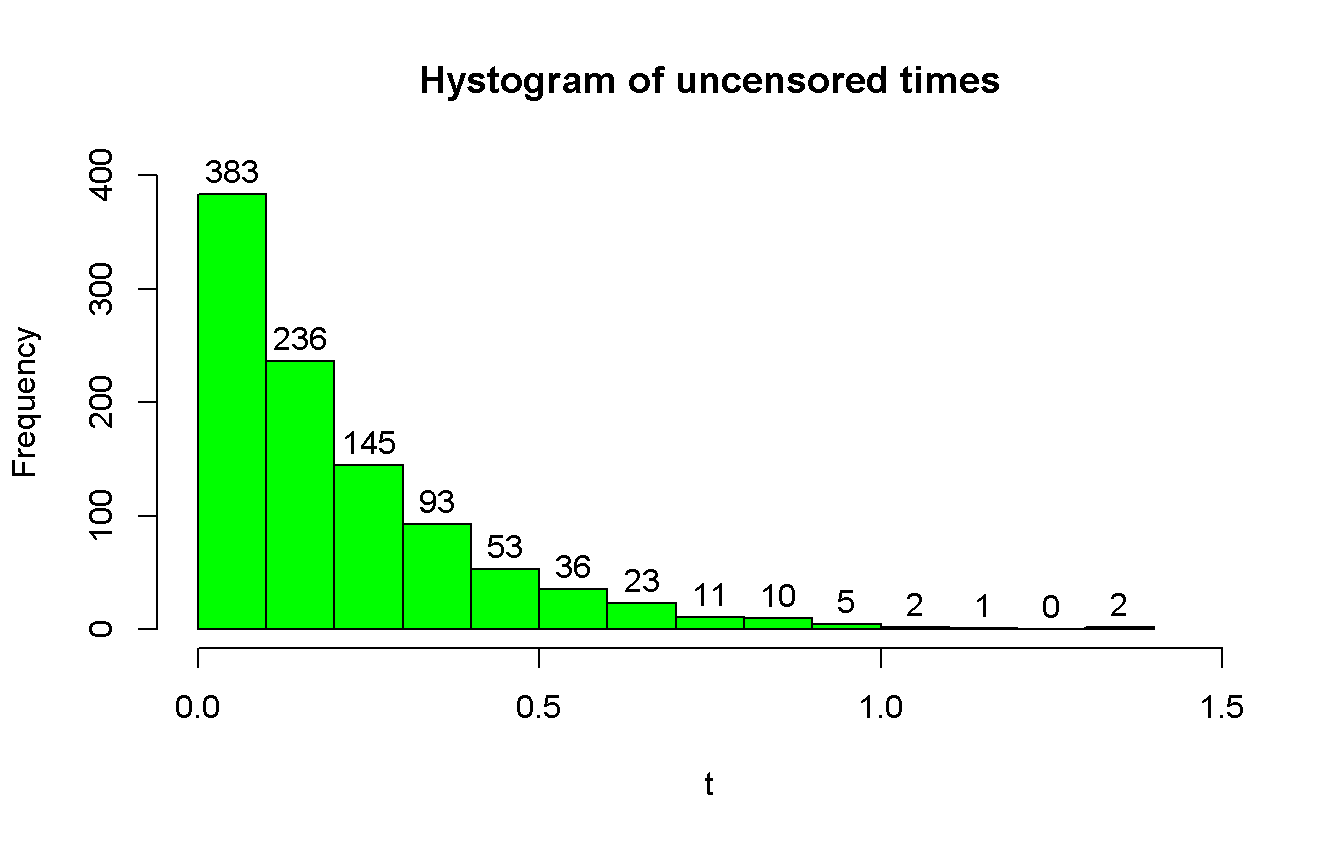
\includegraphics[width=0.5\linewidth]{SuDACDa-notes_files/figure-latex/sim_plots-1}
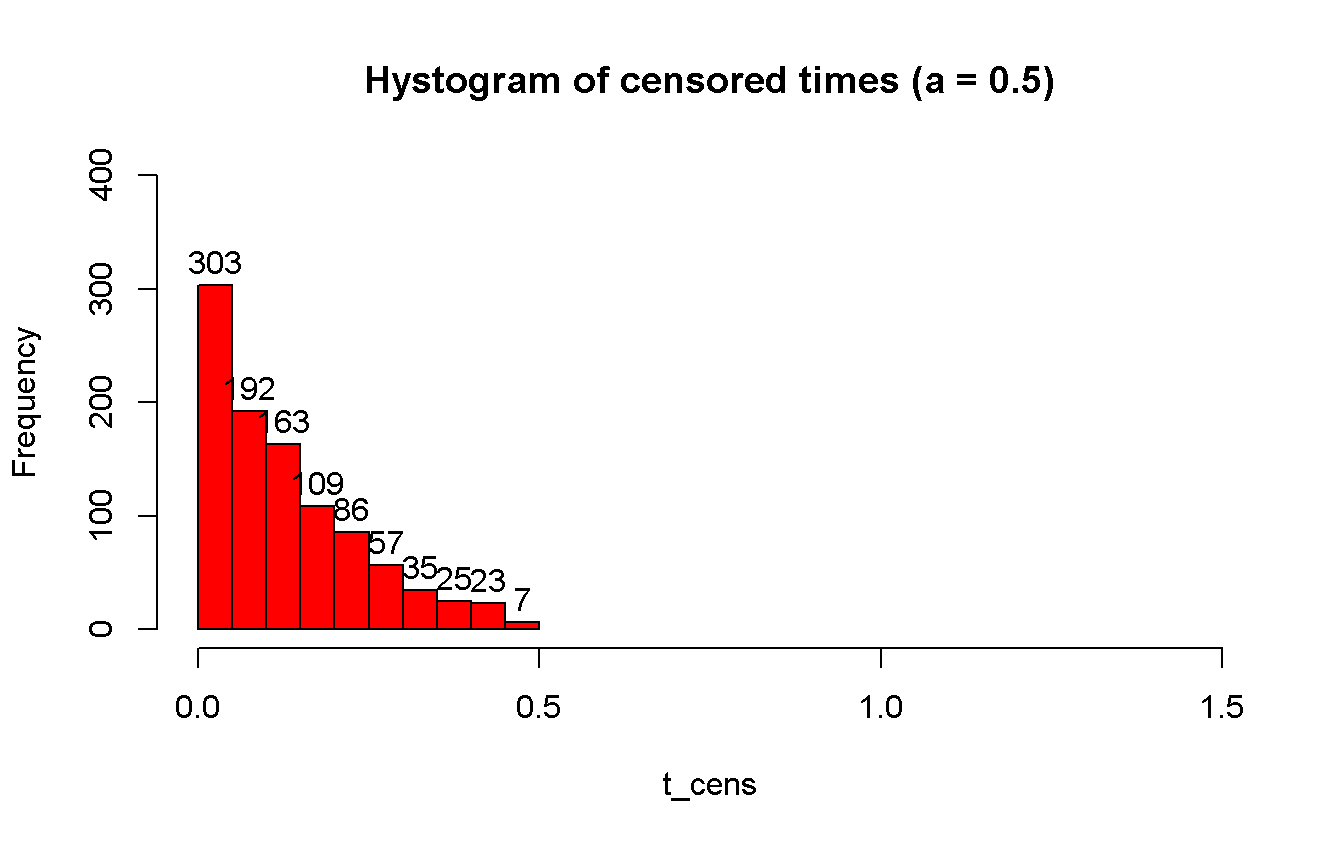
\includegraphics[width=0.5\linewidth]{SuDACDa-notes_files/figure-latex/sim_plots-2}

\begin{enumerate}
\def\labelenumi{\arabic{enumi}.}
\setcounter{enumi}{2}
\tightlist
\item
  Parametric estimation of survival function
\end{enumerate}

\begin{itemize}
\tightlist
\item
  Uncensored
\end{itemize}

\begin{Shaded}
\begin{Highlighting}[]
\CommentTok{# `?survreg` := "Regression for a Parametric Survival Model"}
\CommentTok{# }
\CommentTok{# R formula: y ~ x <--> math formula: y = f(x)}
\CommentTok{# }
\CommentTok{# Here we want to model the response (labelled time) as they are, without any}
\CommentTok{# furter investigation on the effect on them from some other variable}
\KeywordTok{survreg}\NormalTok{(}\KeywordTok{Surv}\NormalTok{(t, status_no_cens) ~}\StringTok{ }\DecValTok{1}\NormalTok{,}
  \DataTypeTok{dist =} \StringTok{'exponential'}
\NormalTok{) %>%}
\StringTok{  }\NormalTok{summary     }\CommentTok{# here `summary()` add some more statistics to the standard output}
\end{Highlighting}
\end{Shaded}

\begin{verbatim}
## 
## Call:
## survreg(formula = Surv(t, status_no_cens) ~ 1, dist = "exponential")
##             Value Std. Error   z p
## (Intercept) -1.61     0.0316 -51 0
## 
## Scale fixed at 1 
## 
## Exponential distribution
## Loglik(model)= 611.6   Loglik(intercept only)= 611.6
## Number of Newton-Raphson Iterations: 4 
## n= 1000
\end{verbatim}

\begin{itemize}
\tightlist
\item
  Censored
\end{itemize}

\begin{Shaded}
\begin{Highlighting}[]
\KeywordTok{survreg}\NormalTok{(}\KeywordTok{Surv}\NormalTok{(t_cens, status_cens) ~}\StringTok{ }\DecValTok{1}\NormalTok{,}
  \DataTypeTok{dist =} \StringTok{'exponential'}
\NormalTok{) %>%}
\StringTok{  }\NormalTok{summary}
\end{Highlighting}
\end{Shaded}

\begin{verbatim}
## 
## Call:
## survreg(formula = Surv(t_cens, status_cens) ~ 1, dist = "exponential")
##             Value Std. Error     z p
## (Intercept) -1.65      0.039 -42.3 0
## 
## Scale fixed at 1 
## 
## Exponential distribution
## Loglik(model)= 427.7   Loglik(intercept only)= 427.7
## Number of Newton-Raphson Iterations: 4 
## n= 1000
\end{verbatim}

\begin{enumerate}
\def\labelenumi{\arabic{enumi}.}
\setcounter{enumi}{3}
\tightlist
\item
  Non parametric estimation of survival and the distribution functions
\end{enumerate}

\begin{itemize}
\tightlist
\item
  Uncensored
\end{itemize}

\begin{Shaded}
\begin{Highlighting}[]
\CommentTok{# `?survfit` := "Create survival curves"}
\KeywordTok{survfit}\NormalTok{(}\KeywordTok{Surv}\NormalTok{(t, status_no_cens) ~}\StringTok{ }\DecValTok{1}\NormalTok{)}
\end{Highlighting}
\end{Shaded}

\begin{verbatim}
## Call: survfit(formula = Surv(t, status_no_cens) ~ 1)
## 
##        n   events   median  0.95LCL  0.95UCL 
## 1000.000 1000.000    0.134    0.123    0.152
\end{verbatim}

\begin{Shaded}
\begin{Highlighting}[]
\CommentTok{# Here we would like to compare to approach to survival plots:}
\CommentTok{# 1. Using the packege _survival_, so the standard one}
\CommentTok{# 2. Uisng the package _rms_, a comprehensive package for regression analyses}

\CommentTok{# Using survival `plot` provided by the _survival_ package}
\CommentTok{# (`?survival:::plot.survfit`), we can continue to}
\CommentTok{# use the `survfit()` function for nonparametric survival estimation from the}
\CommentTok{# same _survival_ package}
\KeywordTok{survfit}\NormalTok{(}\KeywordTok{Surv}\NormalTok{(t, status_no_cens) ~}\StringTok{ }\DecValTok{1}\NormalTok{) %>%}\StringTok{ }
\StringTok{  }\KeywordTok{plot}\NormalTok{(}
    \DataTypeTok{xlim     =} \KeywordTok{c}\NormalTok{(}\DecValTok{0}\NormalTok{, }\FloatTok{1.55}\NormalTok{),}
    \DataTypeTok{conf.int  =} \OtherTok{TRUE}\NormalTok{,}
    \DataTypeTok{mark.time =} \OtherTok{TRUE}\NormalTok{,}
    \DataTypeTok{col       =} \StringTok{'green'}\NormalTok{,}
    \DataTypeTok{main      =} \StringTok{'Uncensored --- survival'}
\NormalTok{)}


\CommentTok{# Using the survplot from the _rms_ package (`survplot`), we have to switch to}
\CommentTok{# the `npsurv()` function for nonparametric survival estimation from the _rms_}
\CommentTok{# package}
\KeywordTok{npsurv}\NormalTok{(}\KeywordTok{Surv}\NormalTok{(t, status_no_cens) ~}\StringTok{ }\DecValTok{1}\NormalTok{) %>%}\StringTok{ }
\StringTok{  }\KeywordTok{survplot}\NormalTok{(}
    \DataTypeTok{xlim     =} \KeywordTok{c}\NormalTok{(}\DecValTok{0}\NormalTok{, }\FloatTok{1.5}\NormalTok{),}
    \DataTypeTok{conf.int =} \OtherTok{TRUE}\NormalTok{,}
    \DataTypeTok{n.risk   =} \OtherTok{TRUE}\NormalTok{,}
    \DataTypeTok{col      =} \StringTok{'green'}
\NormalTok{)}
\KeywordTok{title}\NormalTok{(}\DataTypeTok{main =} \StringTok{'Uncensored --- rms'}\NormalTok{) }\CommentTok{# unfortunally survplot do not have an}
                                   \CommentTok{# integrated option for the title...}
\end{Highlighting}
\end{Shaded}

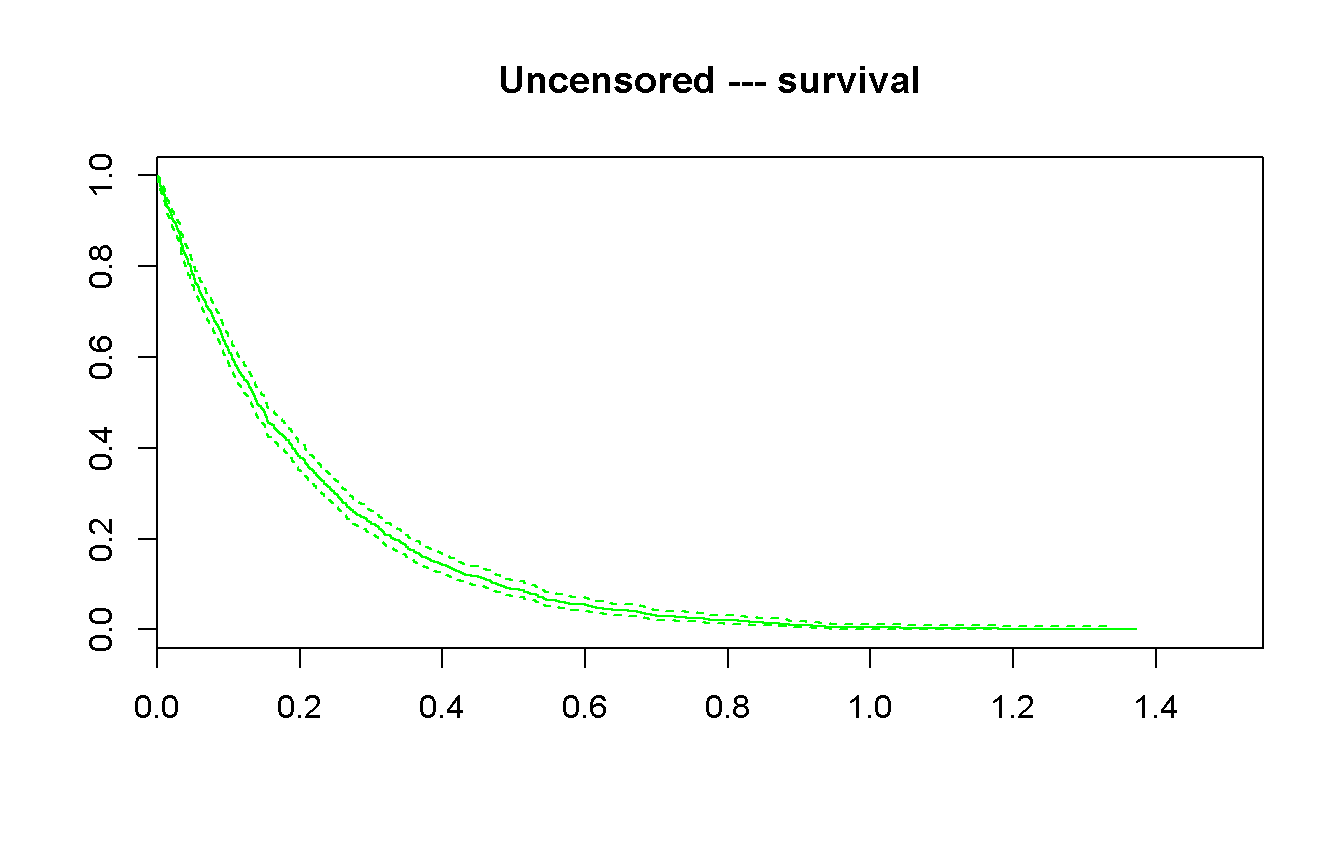
\includegraphics{SuDACDa-notes_files/figure-latex/survfit_nocens-1.pdf}
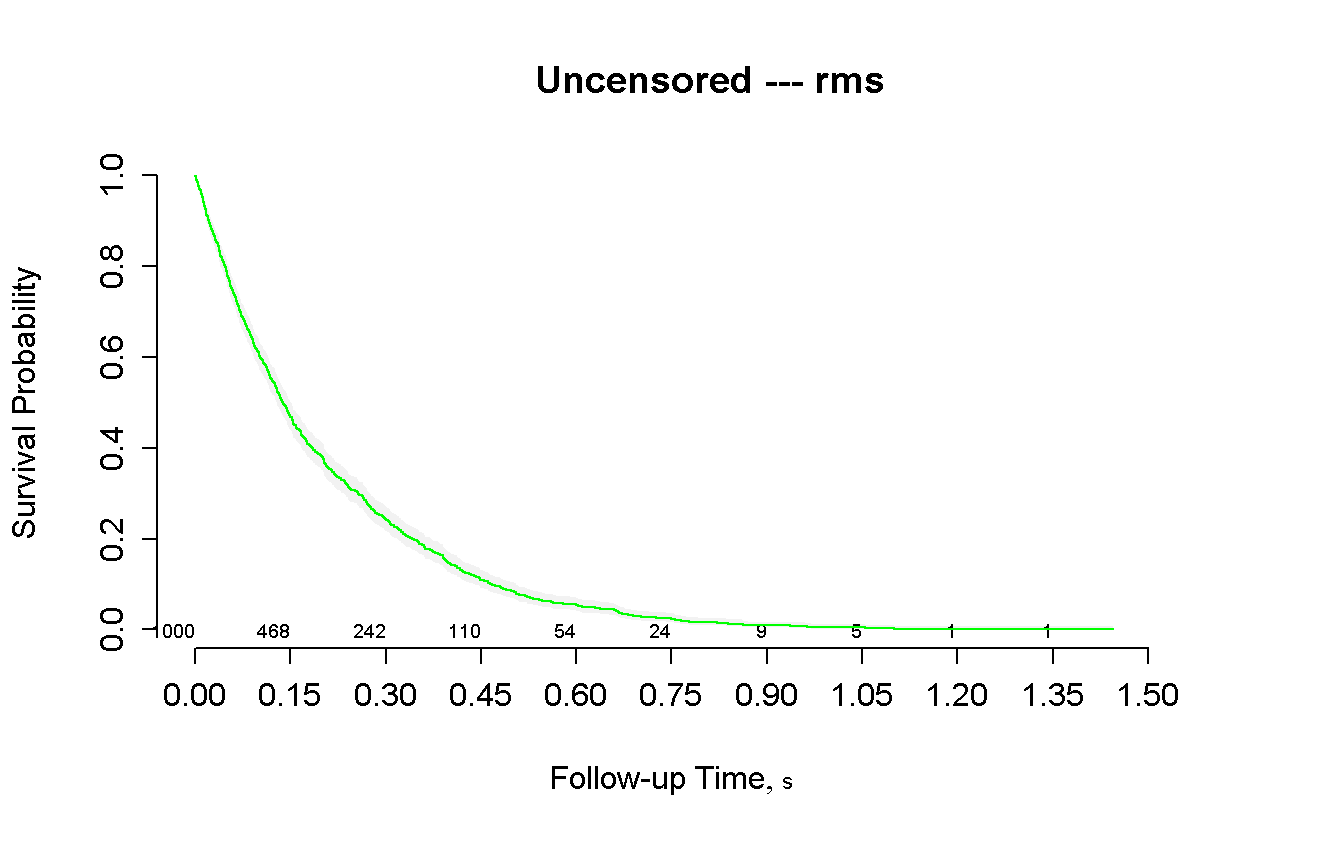
\includegraphics{SuDACDa-notes_files/figure-latex/survfit_nocens-2.pdf}

\begin{itemize}
\tightlist
\item
  censored
\end{itemize}

\begin{Shaded}
\begin{Highlighting}[]
\KeywordTok{survfit}\NormalTok{(}\KeywordTok{Surv}\NormalTok{(t_cens, status_cens) ~}\StringTok{ }\DecValTok{1}\NormalTok{)}
\end{Highlighting}
\end{Shaded}

\begin{verbatim}
## Call: survfit(formula = Surv(t_cens, status_cens) ~ 1)
## 
##        n   events   median  0.95LCL  0.95UCL 
## 1000.000  657.000    0.132    0.122    0.151
\end{verbatim}

\begin{Shaded}
\begin{Highlighting}[]
\KeywordTok{survfit}\NormalTok{(}\KeywordTok{Surv}\NormalTok{(t_cens, status_cens) ~}\StringTok{ }\DecValTok{1}\NormalTok{) %>%}
\StringTok{  }\KeywordTok{plot}\NormalTok{(}
    \DataTypeTok{xlim     =} \KeywordTok{c}\NormalTok{(}\DecValTok{0}\NormalTok{, }\FloatTok{0.55}\NormalTok{),}
    \DataTypeTok{conf.int  =} \OtherTok{TRUE}\NormalTok{,}
    \DataTypeTok{mark.time =} \OtherTok{TRUE}\NormalTok{,}
    \DataTypeTok{col      =} \StringTok{'red'}\NormalTok{,}
    \DataTypeTok{main      =} \StringTok{'Censored (a = 0.5)'}
\NormalTok{)}

\KeywordTok{npsurv}\NormalTok{(}\KeywordTok{Surv}\NormalTok{(t_cens, status_cens) ~}\StringTok{ }\DecValTok{1}\NormalTok{) %>%}\StringTok{ }
\StringTok{  }\KeywordTok{survplot}\NormalTok{(}
    \DataTypeTok{xlim     =} \KeywordTok{c}\NormalTok{(}\DecValTok{0}\NormalTok{, }\FloatTok{0.5}\NormalTok{),}
    \DataTypeTok{conf.int =} \OtherTok{TRUE}\NormalTok{,}
    \DataTypeTok{n.risk   =} \OtherTok{TRUE}\NormalTok{,}
    \DataTypeTok{col      =} \StringTok{'red'}
\NormalTok{)}
\KeywordTok{title}\NormalTok{(}\DataTypeTok{main =} \StringTok{'Censored (a = 0.5) --- rms'}\NormalTok{)}
\end{Highlighting}
\end{Shaded}

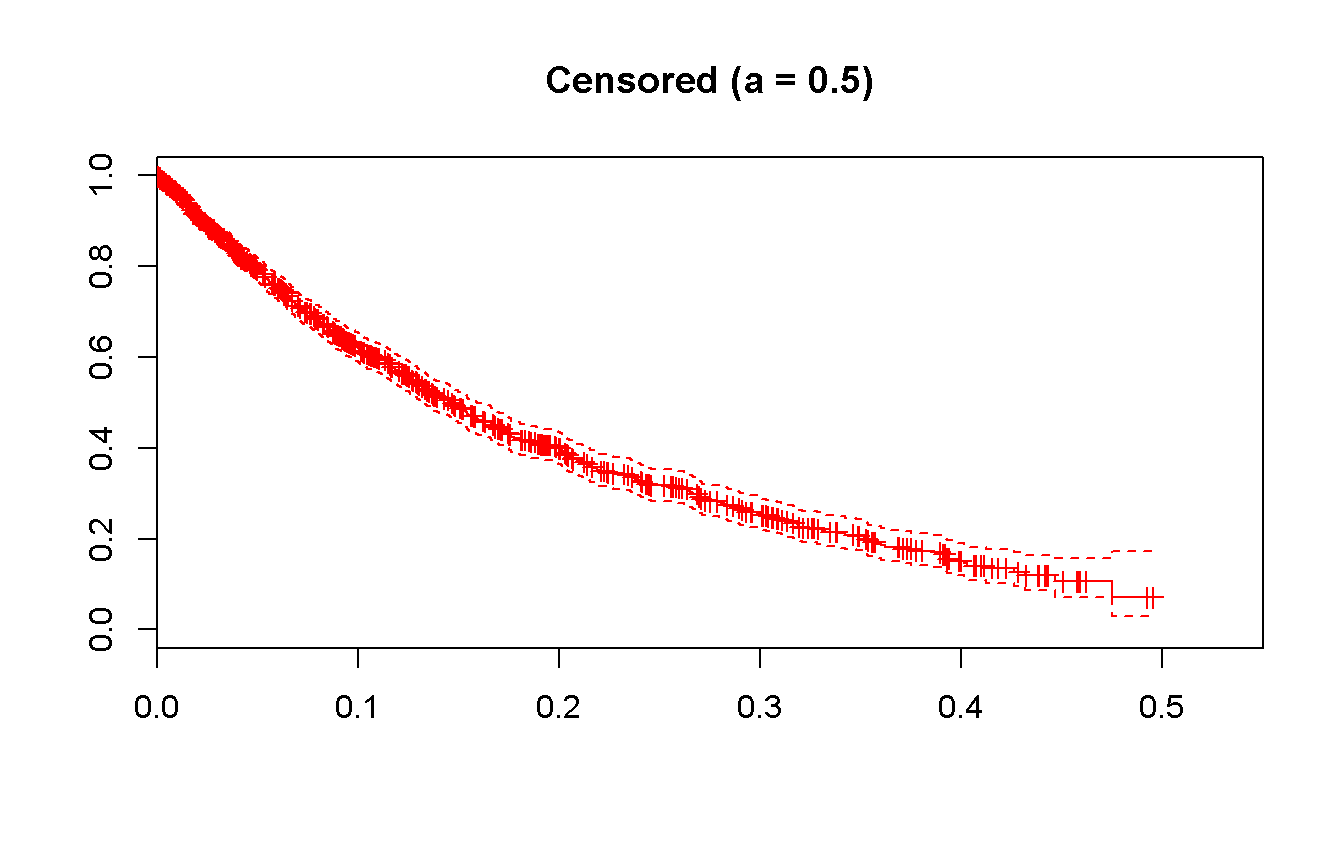
\includegraphics{SuDACDa-notes_files/figure-latex/survfit_cens-1.pdf}
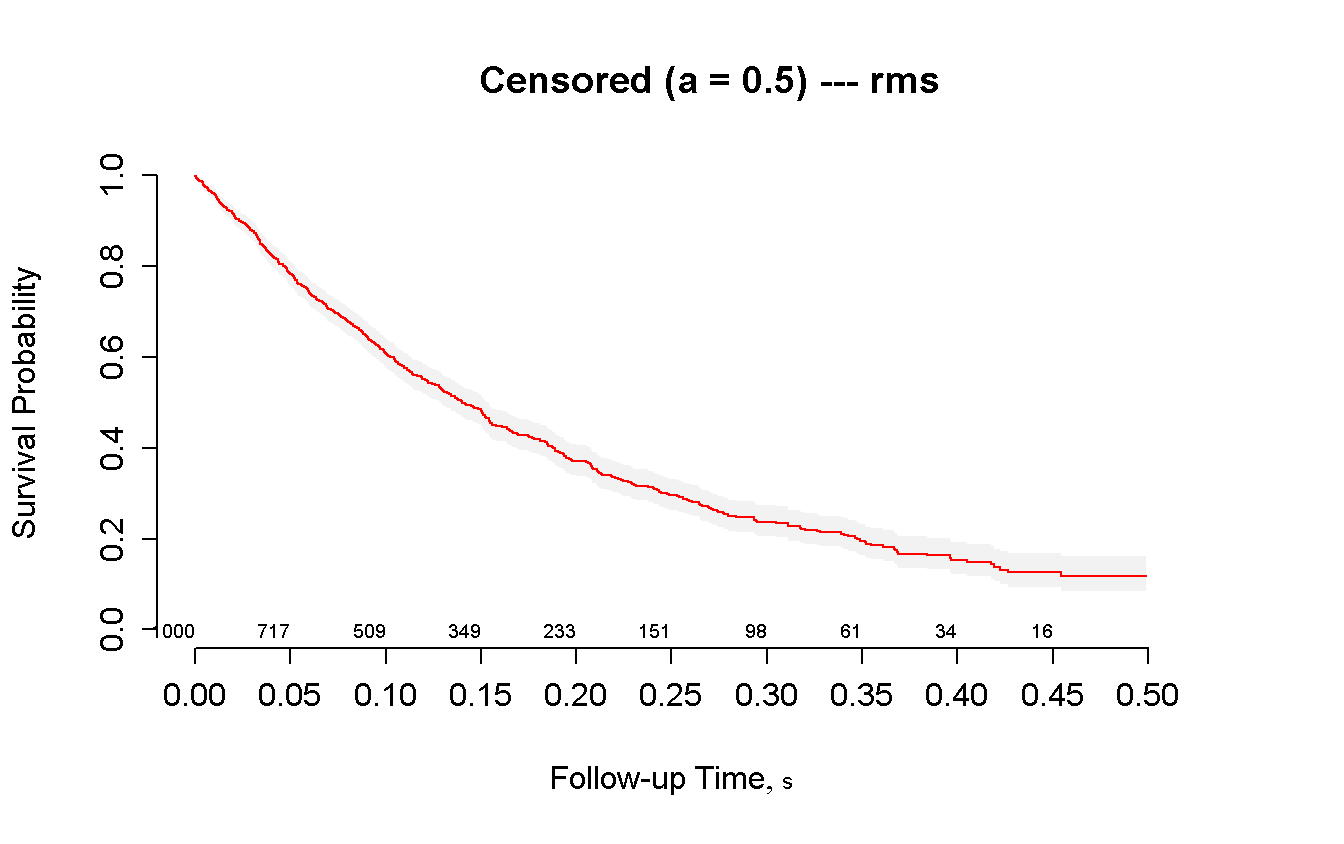
\includegraphics{SuDACDa-notes_files/figure-latex/survfit_cens-2.pdf}

\section{\texorpdfstring{\texttt{mgus} data from \textbf{survival}
package}{mgus data from survival package}}\label{mgus-data-from-survival-package}

\begin{enumerate}
\def\labelenumi{\arabic{enumi}.}
\tightlist
\item
  Load and explore data
\end{enumerate}

\begin{Shaded}
\begin{Highlighting}[]
\KeywordTok{data}\NormalTok{(mgus)                                                                }\CommentTok{# load}
\KeywordTok{head}\NormalTok{(mgus)                                                       }\CommentTok{# first 10 rows}
\end{Highlighting}
\end{Shaded}

\begin{verbatim}
##   id age    sex dxyr pcdx pctime futime death alb creat  hgb mspike
## 1  1  78 female   68 <NA>     NA    748     1 2.8   1.2 11.5    2.0
## 2  2  73 female   66   LP   1310   6751     1  NA    NA   NA    1.3
## 3  3  87   male   68 <NA>     NA    277     1 2.2   1.1 11.2    1.3
## 4  4  86   male   69 <NA>     NA   1815     1 2.8   1.3 15.3    1.8
## 5  5  74 female   68 <NA>     NA   2587     1 3.0   0.8  9.8    1.4
## 6  6  81   male   68 <NA>     NA    563     1 2.9   0.9 11.5    1.8
\end{verbatim}

\begin{Shaded}
\begin{Highlighting}[]
\KeywordTok{dim}\NormalTok{(mgus)                                              }\CommentTok{# number of rows and cols}
\end{Highlighting}
\end{Shaded}

\begin{verbatim}
## [1] 241  12
\end{verbatim}

\begin{Shaded}
\begin{Highlighting}[]
\KeywordTok{names}\NormalTok{(mgus)                                                }\CommentTok{# name of the columns}
\end{Highlighting}
\end{Shaded}

\begin{verbatim}
##  [1] "id"     "age"    "sex"    "dxyr"   "pcdx"   "pctime" "futime"
##  [8] "death"  "alb"    "creat"  "hgb"    "mspike"
\end{verbatim}

\begin{Shaded}
\begin{Highlighting}[]
\KeywordTok{str}\NormalTok{(mgus)                                   }\CommentTok{# R internal structure of the object}
\end{Highlighting}
\end{Shaded}

\begin{verbatim}
## 'data.frame':    241 obs. of  12 variables:
##  $ id    : num  1 2 3 4 5 6 7 8 9 10 ...
##  $ age   : atomic  78 73 87 86 74 81 72 79 85 58 ...
##   ..- attr(*, "label")= chr "AGE AT date_on"
##  $ sex   : Factor w/ 2 levels "female","male": 1 1 2 2 1 2 1 1 1 2 ...
##   ..- attr(*, "label")= chr "Sex"
##  $ dxyr  : num  68 66 68 69 68 68 68 69 70 65 ...
##  $ pcdx  : Factor w/ 4 levels "AM","LP","MA",..: NA 2 NA NA NA NA NA NA NA NA ...
##  $ pctime: atomic  NA 1310 NA NA NA NA NA NA NA NA ...
##   ..- attr(*, "label")= chr "Progression to Group 4 (days)"
##  $ futime: atomic  748 6751 277 1815 2587 ...
##   ..- attr(*, "label")= chr "Follow-Up Time"
##  $ death : num  1 1 1 1 1 1 1 1 1 1 ...
##  $ alb   : atomic  2.8 NA 2.2 2.8 3 2.9 3 3.1 3.2 3.5 ...
##   ..- attr(*, "label")= chr "Serum Albumin"
##  $ creat : atomic  1.2 NA 1.1 1.3 0.8 0.9 0.8 0.8 1 1 ...
##   ..- attr(*, "label")= chr "Serum Creatinine"
##  $ hgb   : atomic  11.5 NA 11.2 15.3 9.8 11.5 13.5 15.5 12.4 14.8 ...
##   ..- attr(*, "label")= chr "Hemoglobin"
##  $ mspike: atomic  2 1.3 1.3 1.8 1.4 1.8 1.3 1.4 1.5 2.2 ...
##   ..- attr(*, "label")= chr "Serum M-Spike"
##  - attr(*, "formats")=List of 1
##   ..$ death:List of 2
##   .. ..$ values: num  0 1
##   .. ..$ labels: chr  "Alive" "Dead"
\end{verbatim}

\begin{Shaded}
\begin{Highlighting}[]
\KeywordTok{summary}\NormalTok{(mgus)                                              }\CommentTok{# summary from base R}
\end{Highlighting}
\end{Shaded}

\begin{verbatim}
##        id           age            sex           dxyr        pcdx    
##  Min.   :  1   Min.   :34.00   female:104   Min.   :56.0   AM  :  8  
##  1st Qu.: 61   1st Qu.:55.00   male  :137   1st Qu.:66.0   LP  :  5  
##  Median :121   Median :63.00                Median :68.0   MA  :  7  
##  Mean   :121   Mean   :62.87                Mean   :67.4   MM  : 44  
##  3rd Qu.:181   3rd Qu.:72.00                3rd Qu.:70.0   NA's:177  
##  Max.   :241   Max.   :90.00                Max.   :73.0             
##                                                                      
##      pctime          futime          death             alb       
##  Min.   :  365   Min.   :    6   Min.   :0.0000   Min.   :1.800  
##  1st Qu.: 2469   1st Qu.: 2422   1st Qu.:1.0000   1st Qu.:2.900  
##  Median : 3778   Median : 5022   Median :1.0000   Median :3.200  
##  Mean   : 4342   Mean   : 5425   Mean   :0.9336   Mean   :3.204  
##  3rd Qu.: 5750   3rd Qu.: 8264   3rd Qu.:1.0000   3rd Qu.:3.500  
##  Max.   :11685   Max.   :14325   Max.   :1.0000   Max.   :5.100  
##  NA's   :177                                      NA's   :31     
##      creat            hgb            mspike     
##  Min.   :0.600   Min.   : 7.40   Min.   :0.300  
##  1st Qu.:0.900   1st Qu.:12.20   1st Qu.:1.500  
##  Median :1.000   Median :13.20   Median :1.700  
##  Mean   :1.095   Mean   :13.15   Mean   :1.764  
##  3rd Qu.:1.100   3rd Qu.:14.50   3rd Qu.:2.000  
##  Max.   :6.400   Max.   :16.60   Max.   :3.200  
##  NA's   :43      NA's   :1
\end{verbatim}

\begin{Shaded}
\begin{Highlighting}[]
\KeywordTok{describe}\NormalTok{(mgus)   }\CommentTok{# more comprehensive description from _Hisc_ package, loaded by}
\end{Highlighting}
\end{Shaded}

\begin{verbatim}
## mgus 
## 
##  12  Variables      241  Observations
## ---------------------------------------------------------------------------
## id 
##        n  missing distinct     Info     Mean      Gmd      .05      .10 
##      241        0      241        1      121    80.67       13       25 
##      .25      .50      .75      .90      .95 
##       61      121      181      217      229 
## 
## lowest :   1   2   3   4   5, highest: 237 238 239 240 241
## ---------------------------------------------------------------------------
## age : AGE AT date_on 
##        n  missing distinct     Info     Mean      Gmd      .05      .10 
##      241        0       53    0.999    62.87    13.42       44       48 
##      .25      .50      .75      .90      .95 
##       55       63       72       78       81 
## 
## lowest : 34 35 36 37 38, highest: 84 85 86 87 90
## ---------------------------------------------------------------------------
## sex : Sex 
##        n  missing distinct 
##      241        0        2 
##                         
## Value      female   male
## Frequency     104    137
## Proportion  0.432  0.568
## ---------------------------------------------------------------------------
## dxyr 
##        n  missing distinct     Info     Mean      Gmd      .05      .10 
##      241        0       17     0.97     67.4    3.073       61       63 
##      .25      .50      .75      .90      .95 
##       66       68       70       70       70 
##                                                                       
## Value         56    58    59    60    61    62    63    64    65    66
## Frequency      1     1     5     5     2     7     7    10    10    18
## Proportion 0.004 0.004 0.021 0.021 0.008 0.029 0.029 0.041 0.041 0.075
##                                                     
## Value         67    68    69    70    71    72    73
## Frequency     24    40    45    62     2     1     1
## Proportion 0.100 0.166 0.187 0.257 0.008 0.004 0.004
## ---------------------------------------------------------------------------
## pcdx 
##        n  missing distinct 
##       64      177        4 
##                                   
## Value         AM    LP    MA    MM
## Frequency      8     5     7    44
## Proportion 0.125 0.078 0.109 0.688
## ---------------------------------------------------------------------------
## pctime : Progression to Group 4 (days) 
##        n  missing distinct     Info     Mean      Gmd      .05      .10 
##       64      177       63        1     4342     3030     1223     1409 
##      .25      .50      .75      .90      .95 
##     2469     3778     5750     8946    10051 
## 
## lowest :   365   700   954  1218  1249, highest:  9723 10109 10359 11354 11685
## ---------------------------------------------------------------------------
## futime : Follow-Up Time 
##        n  missing distinct     Info     Mean      Gmd      .05      .10 
##      241        0      237        1     5425     4222      283      779 
##      .25      .50      .75      .90      .95 
##     2422     5022     8264    11425    12140 
## 
## lowest :     6     7    31    32    39, highest: 12931 13019 13152 14111 14325
## ---------------------------------------------------------------------------
## death 
##        n  missing distinct     Info      Sum     Mean      Gmd 
##      241        0        2    0.186      225   0.9336   0.1245 
## 
## ---------------------------------------------------------------------------
## alb : Serum Albumin 
##        n  missing distinct     Info     Mean      Gmd      .05      .10 
##      210       31       26    0.995    3.204   0.5293      2.3      2.6 
##      .25      .50      .75      .90      .95 
##      2.9      3.2      3.5      3.8      3.9 
## 
## lowest : 1.8 1.9 2.1 2.2 2.3, highest: 4.0 4.1 4.3 4.5 5.1
## ---------------------------------------------------------------------------
## creat : Serum Creatinine 
##        n  missing distinct     Info     Mean      Gmd      .05      .10 
##      198       43       19    0.978    1.095     0.39    0.700    0.800 
##      .25      .50      .75      .90      .95 
##    0.900    1.000    1.100    1.300    1.615 
##                                                                       
## Value        0.6   0.7   0.8   0.9   1.0   1.1   1.2   1.3   1.4   1.5
## Frequency      4    13    26    42    35    29    18    12     4     4
## Proportion 0.020 0.066 0.131 0.212 0.177 0.146 0.091 0.061 0.020 0.020
##                                                                 
## Value        1.6   1.7   2.0   2.5   2.6   3.5   3.6   3.7   6.4
## Frequency      1     3     1     1     1     1     1     1     1
## Proportion 0.005 0.015 0.005 0.005 0.005 0.005 0.005 0.005 0.005
## ---------------------------------------------------------------------------
## hgb : Hemoglobin 
##        n  missing distinct     Info     Mean      Gmd      .05      .10 
##      240        1       66    0.999    13.15    1.865    10.20    11.09 
##      .25      .50      .75      .90      .95 
##    12.20    13.20    14.50    15.11    15.51 
## 
## lowest :  7.4  7.7  8.4  9.5  9.6, highest: 15.9 16.1 16.2 16.5 16.6
## ---------------------------------------------------------------------------
## mspike : Serum M-Spike 
##        n  missing distinct     Info     Mean      Gmd      .05      .10 
##      241        0       23    0.993    1.764   0.4687      1.1      1.3 
##      .25      .50      .75      .90      .95 
##      1.5      1.7      2.0      2.3      2.5 
## 
## lowest : 0.3 0.8 0.9 1.0 1.1, highest: 2.5 2.6 2.7 2.9 3.2
## ---------------------------------------------------------------------------
\end{verbatim}

\begin{Shaded}
\begin{Highlighting}[]
                 \CommentTok{# the _rms_ one}

\NormalTok{mgus_df <-}\StringTok{ }\KeywordTok{as_tibble}\NormalTok{(mgus)         }\CommentTok{# tidy data frame (important info printed all}
                                   \CommentTok{# together, and visualization auto-adjusted}
                                   \CommentTok{# to the consol width)}
\NormalTok{mgus_df}
\end{Highlighting}
\end{Shaded}

\begin{verbatim}
## # A tibble: 241 x 12
##       id   age    sex  dxyr   pcdx pctime futime death   alb creat   hgb
##  * <dbl> <dbl> <fctr> <dbl> <fctr>  <dbl>  <dbl> <dbl> <dbl> <dbl> <dbl>
##  1     1    78 female    68   <NA>     NA    748     1   2.8   1.2  11.5
##  2     2    73 female    66     LP   1310   6751     1    NA    NA    NA
##  3     3    87   male    68   <NA>     NA    277     1   2.2   1.1  11.2
##  4     4    86   male    69   <NA>     NA   1815     1   2.8   1.3  15.3
##  5     5    74 female    68   <NA>     NA   2587     1   3.0   0.8   9.8
##  6     6    81   male    68   <NA>     NA    563     1   2.9   0.9  11.5
##  7     7    72 female    68   <NA>     NA   1135     1   3.0   0.8  13.5
##  8     8    79 female    69   <NA>     NA   2016     1   3.1   0.8  15.5
##  9     9    85 female    70   <NA>     NA   2422     1   3.2   1.0  12.4
## 10    10    58   male    65   <NA>     NA   6155     1   3.5   1.0  14.8
## # ... with 231 more rows, and 1 more variables: mspike <dbl>
\end{verbatim}

\begin{enumerate}
\def\labelenumi{\arabic{enumi}.}
\setcounter{enumi}{1}
\tightlist
\item
  Non parametric kaplan-Meyer estimation of the survival function
\end{enumerate}

\begin{itemize}
\tightlist
\item
  Estimate the survival function from randomization overall and
  according to sex.
\end{itemize}

\begin{Shaded}
\begin{Highlighting}[]
\KeywordTok{survfit}\NormalTok{(}\KeywordTok{Surv}\NormalTok{(futime, death) ~}\StringTok{ }\DecValTok{1}\NormalTok{,}
  \DataTypeTok{data =} \NormalTok{mgus_df}
\NormalTok{) %>%}
\StringTok{  }\KeywordTok{plot}\NormalTok{(}
    \DataTypeTok{conf.int  =} \OtherTok{TRUE}\NormalTok{,}
    \DataTypeTok{mark.time =} \OtherTok{TRUE}\NormalTok{,}
    \DataTypeTok{col       =} \StringTok{'blue'}\NormalTok{,}
    \DataTypeTok{main      =} \StringTok{'Survival function for mgus data'}
\NormalTok{)}


\KeywordTok{survfit}\NormalTok{(}\KeywordTok{Surv}\NormalTok{(futime, death) ~}\StringTok{ }\NormalTok{sex,}
  \DataTypeTok{data =} \NormalTok{mgus_df}
\NormalTok{) %>%}
\StringTok{  }\KeywordTok{plot}\NormalTok{(}
    \DataTypeTok{conf.int  =} \OtherTok{TRUE}\NormalTok{,}
    \DataTypeTok{mark.time =} \OtherTok{TRUE}\NormalTok{,}
    \DataTypeTok{main      =} \StringTok{'Survival function for mgus data according to sex'}\NormalTok{,}
    \DataTypeTok{col       =} \KeywordTok{c}\NormalTok{(}\StringTok{'red'}\NormalTok{, }\StringTok{'blue'}\NormalTok{),}
    \DataTypeTok{lty       =} \KeywordTok{c}\NormalTok{(}\DecValTok{2}\NormalTok{, }\DecValTok{3}\NormalTok{)}
\NormalTok{)}
\KeywordTok{legend}\NormalTok{(}
  \DataTypeTok{x =} \DecValTok{10000}\NormalTok{, }\DataTypeTok{y =} \DecValTok{1}\NormalTok{,}
  \DataTypeTok{legend =} \KeywordTok{c}\NormalTok{(}\StringTok{"Female"}\NormalTok{, }\StringTok{"Male"}\NormalTok{),}
  \DataTypeTok{col    =} \KeywordTok{c}\NormalTok{(}\StringTok{'red'}\NormalTok{, }\StringTok{'blue'}\NormalTok{),}
  \DataTypeTok{lty    =} \KeywordTok{c}\NormalTok{(}\DecValTok{2}\NormalTok{, }\DecValTok{3}\NormalTok{)}
\NormalTok{)}
\end{Highlighting}
\end{Shaded}

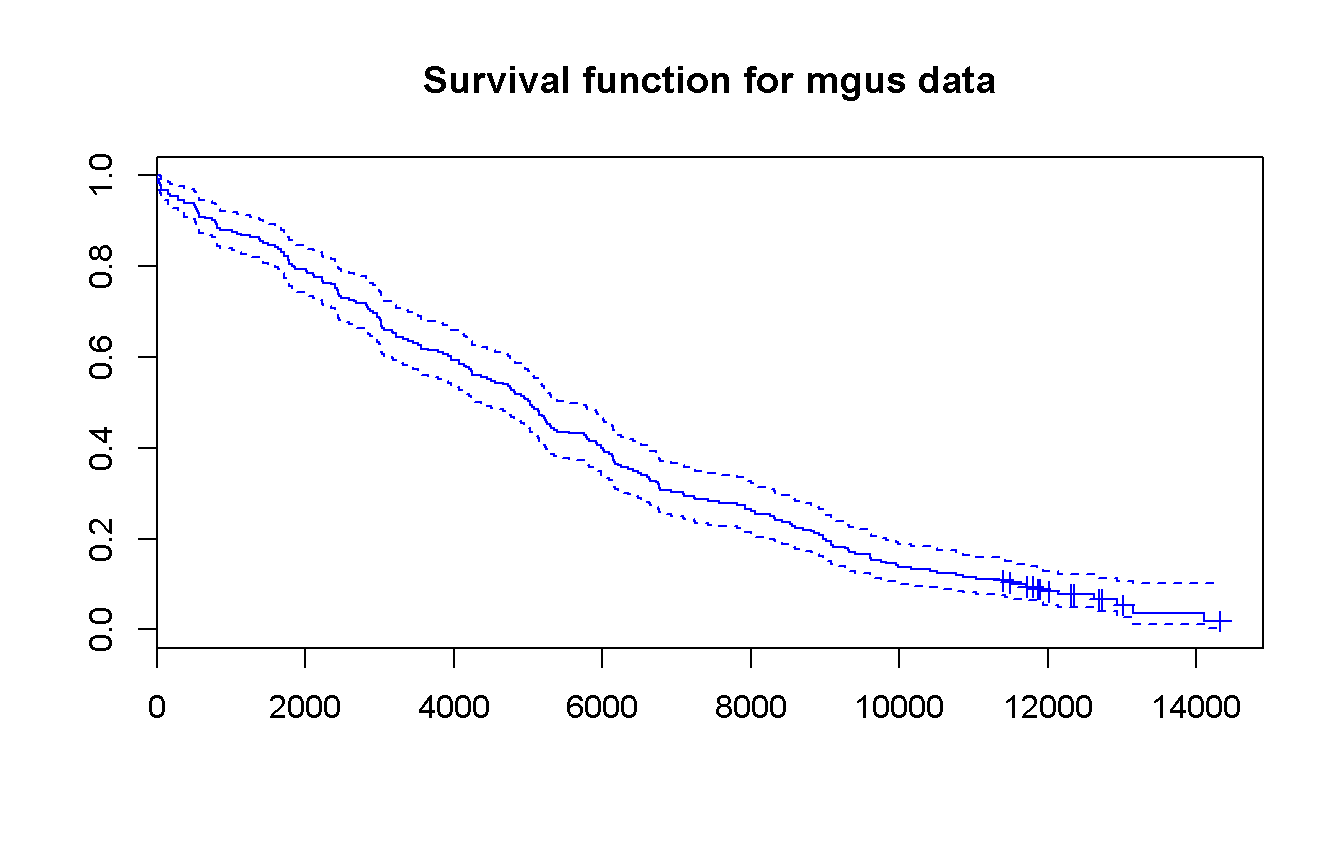
\includegraphics{SuDACDa-notes_files/figure-latex/rmgus_survfit-1.pdf}
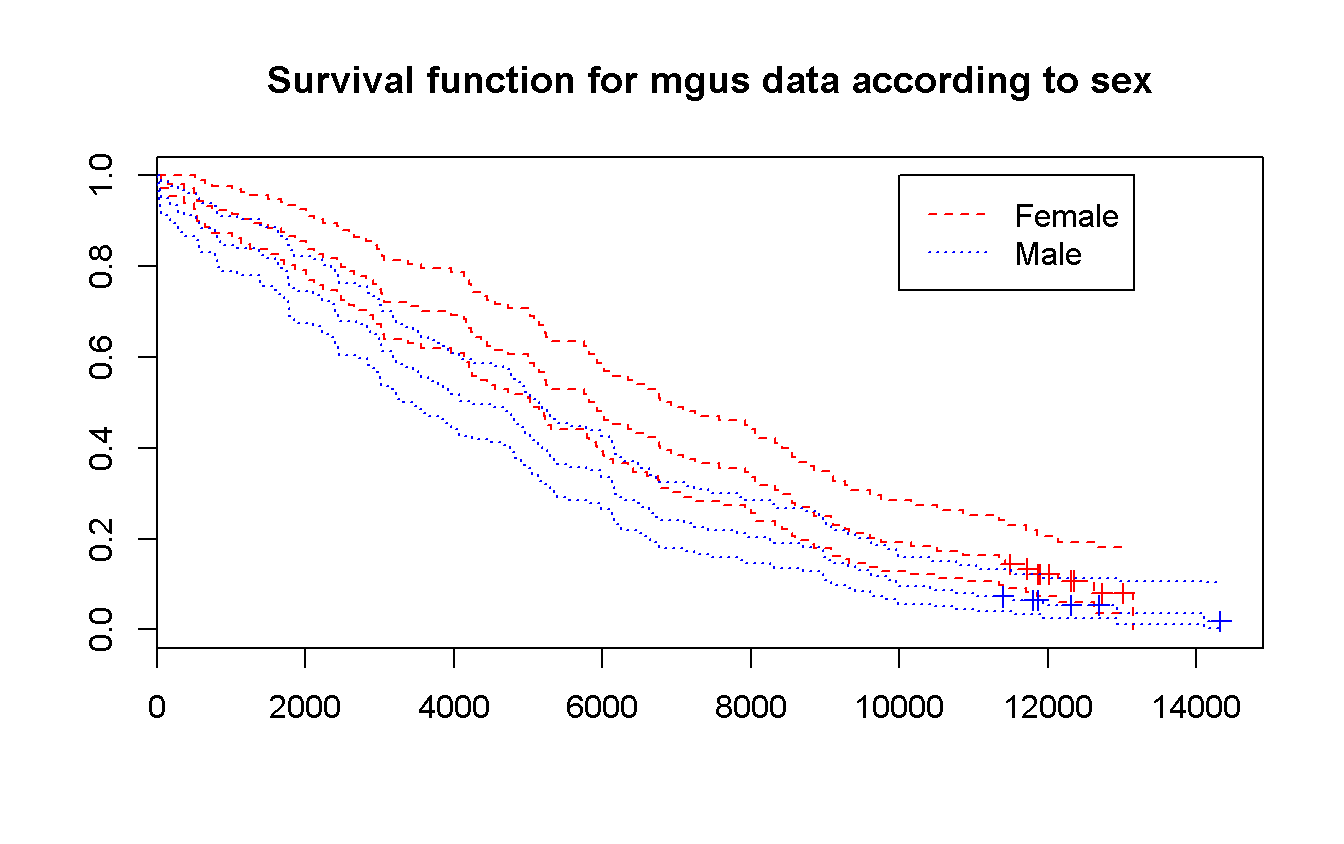
\includegraphics{SuDACDa-notes_files/figure-latex/rmgus_survfit-2.pdf}

\begin{Shaded}
\begin{Highlighting}[]
\CommentTok{# For survival object the package _survminer_ provide ggplot2 plots}
\CommentTok{# (`?ggsurvplot`) which could be very interesting and quite comprehensive.}

\KeywordTok{survfit}\NormalTok{(}\KeywordTok{Surv}\NormalTok{(futime, death) ~}\StringTok{ }\NormalTok{sex,}
  \DataTypeTok{data =} \NormalTok{mgus_df}
\NormalTok{) %>%}\StringTok{ }
\StringTok{  }\KeywordTok{ggsurvplot}\NormalTok{(}
    \DataTypeTok{conf.int            =} \OtherTok{TRUE}\NormalTok{,                      }\CommentTok{# draw confidence intervals}
    \DataTypeTok{pval                =} \OtherTok{TRUE}\NormalTok{,                                    }\CommentTok{# show pvalue}
    \DataTypeTok{pval.method         =} \OtherTok{TRUE}\NormalTok{,                            }\CommentTok{# print the test name}
    \DataTypeTok{title               =} \StringTok{'Survival curves for overall death according to sex.'}\NormalTok{,}
    \DataTypeTok{xlab                =} \StringTok{'Days'}\NormalTok{,}
    \DataTypeTok{legend              =} \StringTok{'right'}\NormalTok{,                             }\CommentTok{# legend position}
    \DataTypeTok{legend.title        =} \StringTok{'Sex'}\NormalTok{,}
    \DataTypeTok{legend.labs         =} \KeywordTok{c}\NormalTok{(}\StringTok{'Female'}\NormalTok{, }\StringTok{'Male'}\NormalTok{),}
    \DataTypeTok{risk.table          =} \OtherTok{TRUE}\NormalTok{,     }\CommentTok{# admits interesting options other than TRUE}
    \DataTypeTok{cumcensor           =} \OtherTok{TRUE}\NormalTok{,}
    \DataTypeTok{cumevents           =} \OtherTok{TRUE}\NormalTok{,}
    \DataTypeTok{pval.size           =} \FloatTok{3.5}\NormalTok{,   }\CommentTok{# from here these are options passed to `ggpar`}
    \DataTypeTok{risk.table.fontsize =} \DecValTok{3}\NormalTok{,     }\CommentTok{# for a better visualization}
    \DataTypeTok{fontsize            =} \DecValTok{3}\NormalTok{,     }\CommentTok{# (auto-explicatives)}
    \DataTypeTok{xscale              =} \FloatTok{30.44}
  \NormalTok{)}
\end{Highlighting}
\end{Shaded}

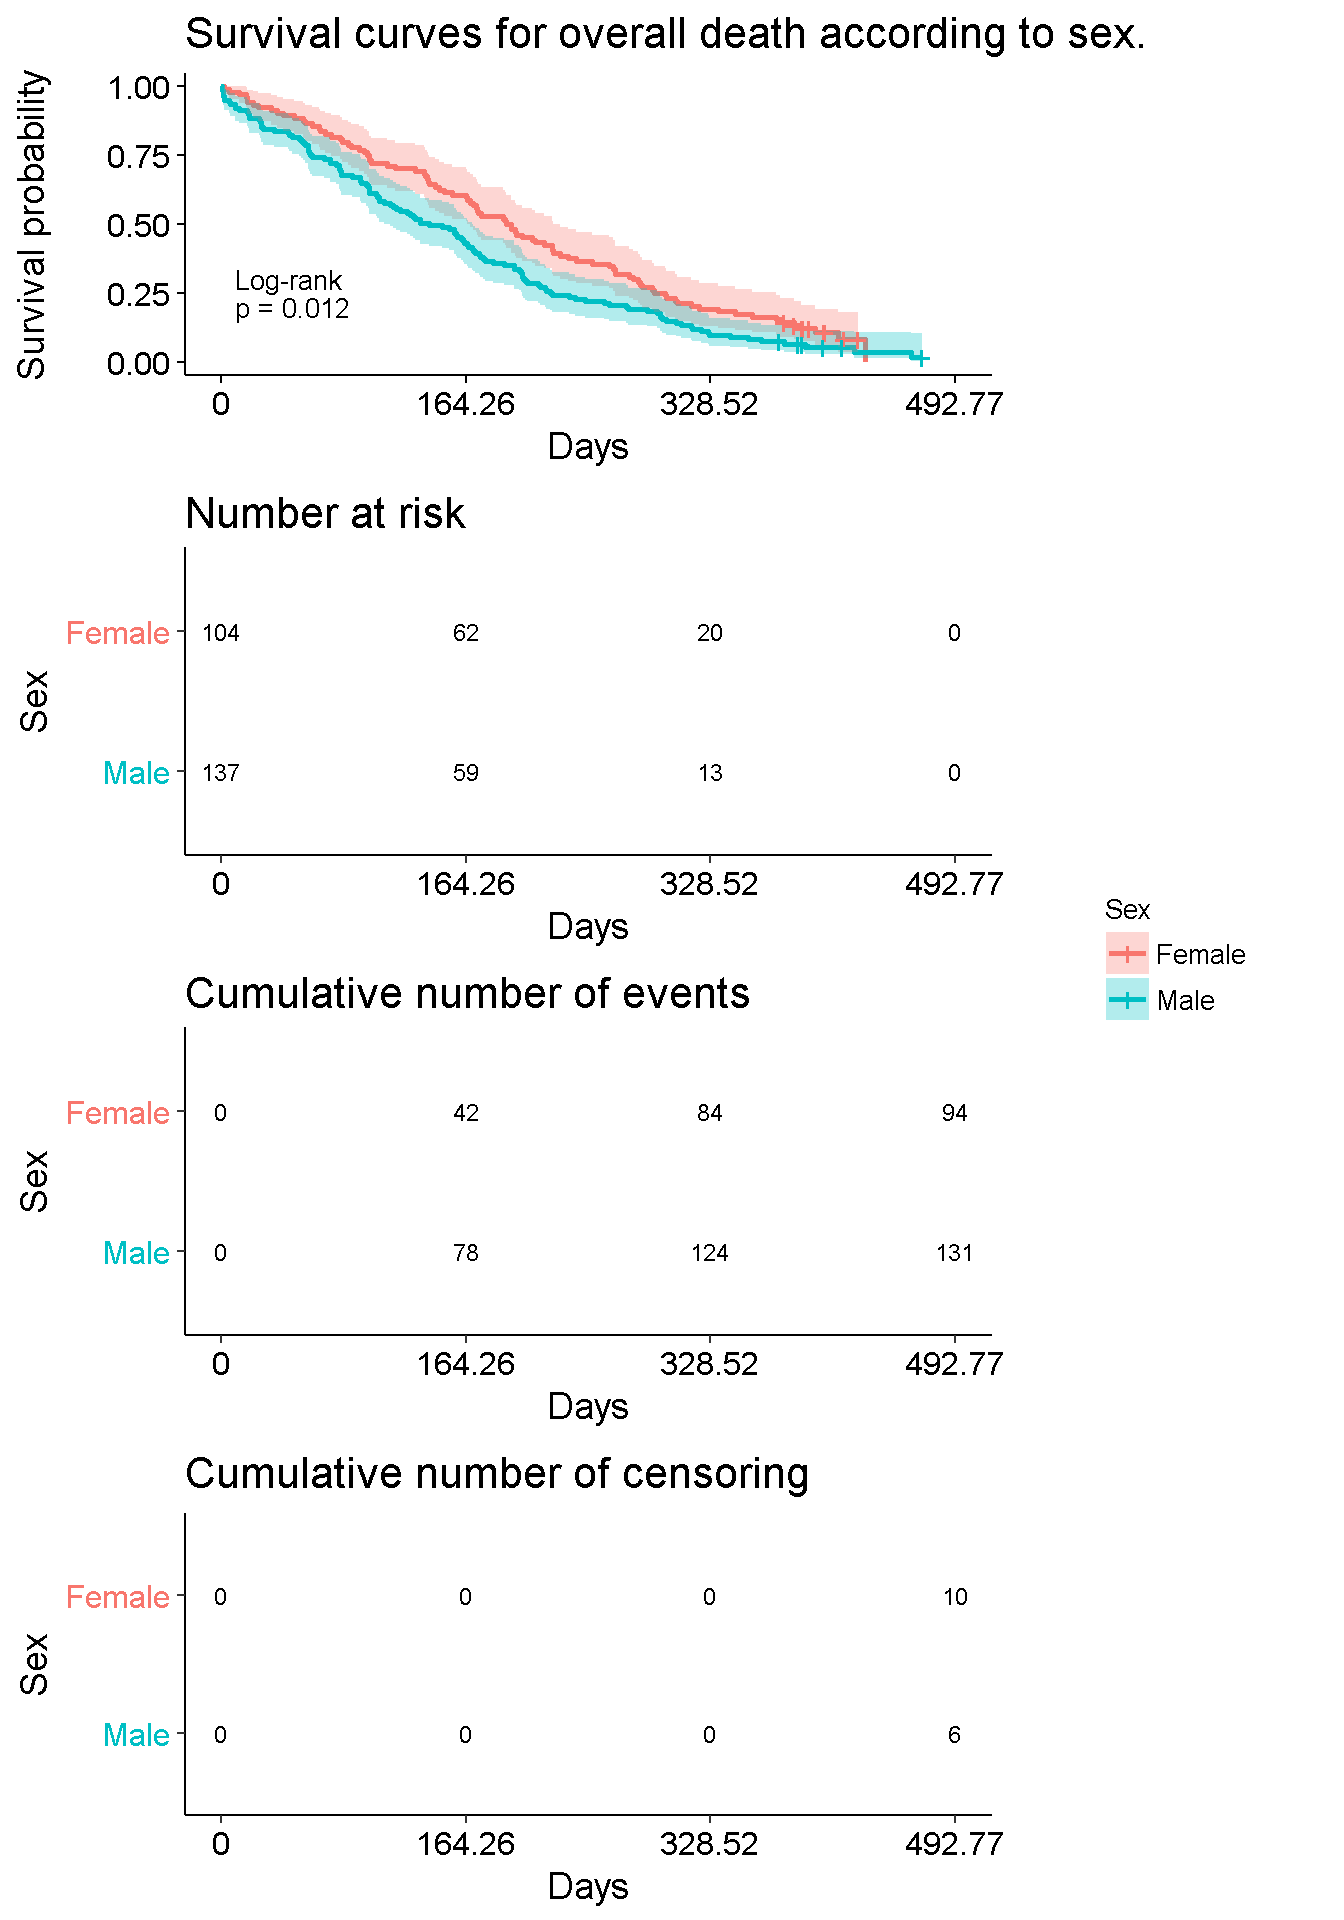
\includegraphics{SuDACDa-notes_files/figure-latex/rmgus_survminer-1.pdf}

\begin{quote}
Note: No female reaches the end of the f-up!
\end{quote}

\begin{itemize}
\tightlist
\item
  Test the effect of sex
\end{itemize}

\begin{Shaded}
\begin{Highlighting}[]
\CommentTok{# Using __survival__ (no plot method is provided for this solution)}
\KeywordTok{survdiff}\NormalTok{(}\KeywordTok{Surv}\NormalTok{(futime, death) ~}\StringTok{ }\NormalTok{sex,}
  \DataTypeTok{data =} \NormalTok{mgus_df}
\NormalTok{)}
\end{Highlighting}
\end{Shaded}

\begin{verbatim}
## Call:
## survdiff(formula = Surv(futime, death) ~ sex, data = mgus_df)
## 
##              N Observed Expected (O-E)^2/E (O-E)^2/V
## sex=female 104       94      113      3.08      6.25
## sex=male   137      131      112      3.08      6.25
## 
##  Chisq= 6.2  on 1 degrees of freedom, p= 0.0124
\end{verbatim}

\begin{Shaded}
\begin{Highlighting}[]
\CommentTok{# using __rms__}
\NormalTok{dd <-}\StringTok{ }\KeywordTok{datadist}\NormalTok{(mgus_df)  }\CommentTok{# To evaluate cph, _rms_ needs this object which simply}
                         \CommentTok{# store statistics about the data.}
                         \CommentTok{# }
                         \CommentTok{# Note: the name of the object (i.e. "dd") has to be }
                         \CommentTok{#       exactly the same as the one specified into the}
                         \CommentTok{#       option set just after the `library(rms)` call.}
                         \CommentTok{#       (See: Chapter settings) }
\NormalTok{cox_model <-}\StringTok{ }\KeywordTok{cph}\NormalTok{(}\KeywordTok{Surv}\NormalTok{(futime, death) ~}\StringTok{ }\NormalTok{sex,}
  \DataTypeTok{data  =} \NormalTok{mgus_df}
\NormalTok{)}

\KeywordTok{summary}\NormalTok{(cox_model)                           }\CommentTok{# return effect size and HR with CI}
\end{Highlighting}
\end{Shaded}

\begin{verbatim}
##              Effects              Response : Surv(futime, death) 
## 
##  Factor            Low High Diff. Effect   S.E.    Lower 0.95 Upper 0.95
##  sex - female:male 2   1    NA    -0.33853 0.13603 -0.60514   -0.071916 
##   Hazard Ratio     2   1    NA     0.71282      NA  0.54600    0.930610
\end{verbatim}

\begin{Shaded}
\begin{Highlighting}[]
\KeywordTok{Predict}\NormalTok{(cox_model) %>%}\StringTok{          }\CommentTok{# Compute predicted values and confidence limits}
\StringTok{                                }\CommentTok{#}
\StringTok{                                }\CommentTok{# Note: pay attention to Title-case "P"redict}
\StringTok{  }\KeywordTok{plot}\NormalTok{(}
    \DataTypeTok{groups =} \StringTok{'sex'}\NormalTok{,}
    \DataTypeTok{anova  =} \KeywordTok{anova}\NormalTok{(cox_model),       }\CommentTok{# Compute and print the $\textbackslash{}chi^2$ statistics}
    \DataTypeTok{pval   =} \OtherTok{TRUE}                    \CommentTok{# print the pvalue }
\NormalTok{)}
\end{Highlighting}
\end{Shaded}

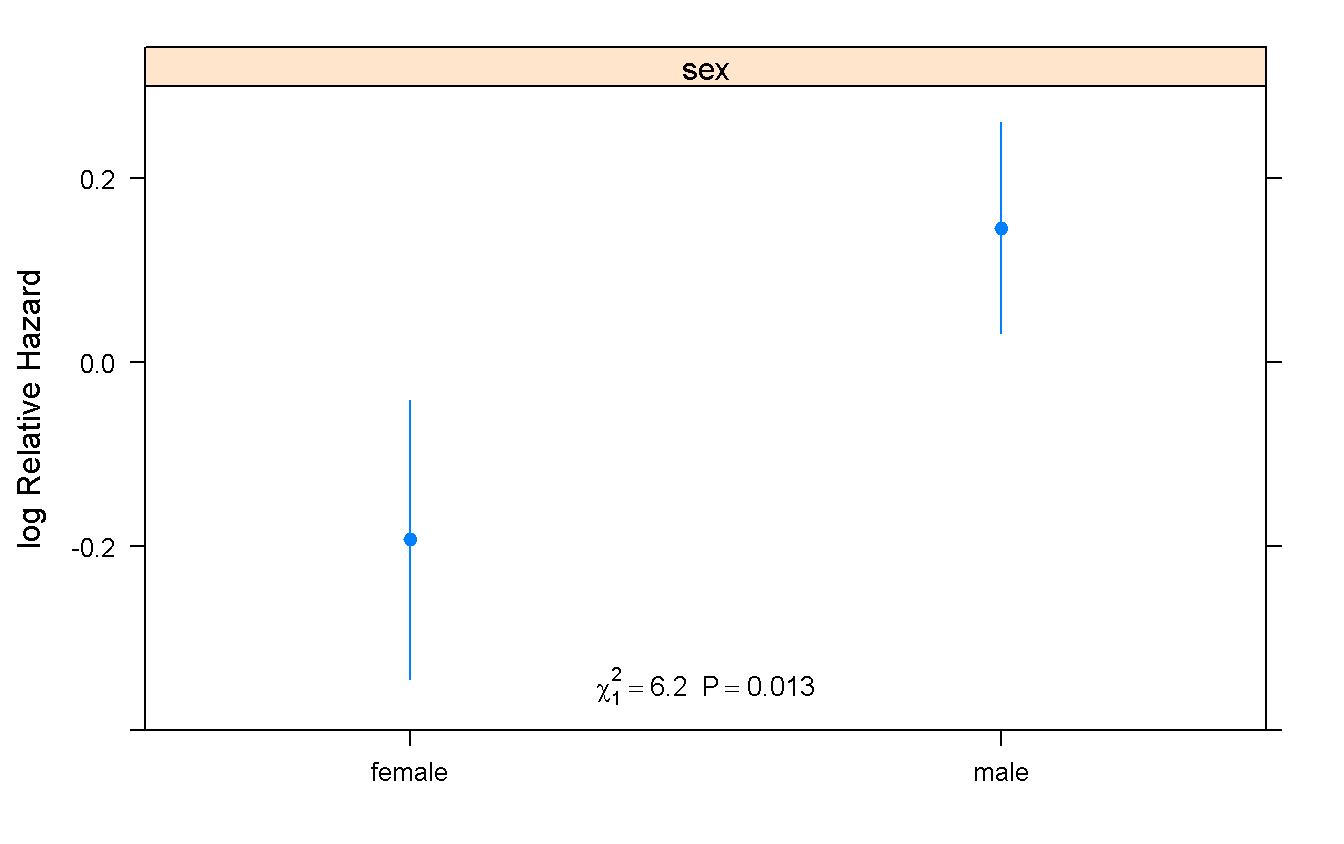
\includegraphics{SuDACDa-notes_files/figure-latex/mgus_survdiff_and_rms-1.pdf}

\section{Non parametric Kalan-Meyer estimation of the survival
function}\label{non-parametric-kalan-meyer-estimation-of-the-survival-function}

\begin{enumerate}
\def\labelenumi{\arabic{enumi}.}
\tightlist
\item
  Let consider a sample of \(n = 500\)
\end{enumerate}

\begin{Shaded}
\begin{Highlighting}[]
\NormalTok{n <-}\StringTok{ }\DecValTok{500}
\end{Highlighting}
\end{Shaded}

\begin{enumerate}
\def\labelenumi{\arabic{enumi}.}
\setcounter{enumi}{1}
\tightlist
\item
  Sumulate the dates of entry in the cohort, from January, 2010 to
  January, 2017
\end{enumerate}

\begin{Shaded}
\begin{Highlighting}[]
\NormalTok{n_days <-}\StringTok{ }\FloatTok{365.25} \NormalTok{*}\StringTok{ }\DecValTok{7}              \CommentTok{# Seven years, taking into account bissextiles}
\NormalTok{time_start <-}\StringTok{ }\KeywordTok{runif}\NormalTok{(}\DataTypeTok{n =} \NormalTok{n,}
  \DataTypeTok{min =} \DecValTok{0}\NormalTok{,}
  \DataTypeTok{max =} \NormalTok{n_days}
\NormalTok{) %>%}\StringTok{ }
\StringTok{  }\KeywordTok{as.Date}\NormalTok{(}\DataTypeTok{origin =} \StringTok{'2010-01-01'}\NormalTok{)}
\end{Highlighting}
\end{Shaded}

\begin{enumerate}
\def\labelenumi{\arabic{enumi}.}
\setcounter{enumi}{2}
\tightlist
\item
  Simulate the dataset of death, assuming exponential death times of
  mean \(2\) years
\end{enumerate}

\begin{Shaded}
\begin{Highlighting}[]
\NormalTok{mean_death_time <-}\StringTok{ }\FloatTok{365.25} \NormalTok{*}\StringTok{ }\DecValTok{2}
\NormalTok{death_t         <-}\StringTok{ }\KeywordTok{rexp}\NormalTok{(n, }\DataTypeTok{rate =} \DecValTok{1} \NormalTok{/}\StringTok{ }\NormalTok{mean_death_time)}
\NormalTok{status_no_cens  <-}\StringTok{ }\KeywordTok{rep}\NormalTok{(}\DecValTok{1}\NormalTok{, n)}
\end{Highlighting}
\end{Shaded}

\begin{enumerate}
\def\labelenumi{\arabic{enumi}.}
\setcounter{enumi}{3}
\tightlist
\item
  Let fix the reference date of the analyses of June, 2017
\end{enumerate}

\begin{Shaded}
\begin{Highlighting}[]
\NormalTok{end_date     <-}\StringTok{ }\KeywordTok{as.Date}\NormalTok{(}\StringTok{'2017-06-01'}\NormalTok{)           }\CommentTok{# Fixed date for the end of f-up}
\NormalTok{death_r_cens <-}\StringTok{ }\KeywordTok{pmin}\NormalTok{(death_t, end_date -}\StringTok{ }\NormalTok{time_start)}
\NormalTok{status_cens  <-}\StringTok{ }\NormalTok{status_no_cens -}\StringTok{ }\NormalTok{(death_t ==}\StringTok{ }\NormalTok{death_r_cens)}
\end{Highlighting}
\end{Shaded}

\begin{enumerate}
\def\labelenumi{\arabic{enumi}.}
\setcounter{enumi}{4}
\tightlist
\item
  Estimate the survival function from randomization
\end{enumerate}

\begin{Shaded}
\begin{Highlighting}[]
\KeywordTok{survfit}\NormalTok{(}\KeywordTok{Surv}\NormalTok{(death_r_cens, status_cens) ~}\StringTok{ }\DecValTok{1}\NormalTok{) %>%}\StringTok{ }
\StringTok{  }\KeywordTok{plot}\NormalTok{(}
    \DataTypeTok{conf.int  =} \OtherTok{TRUE}\NormalTok{,}
    \DataTypeTok{mark.time =} \OtherTok{TRUE}\NormalTok{,}
    \DataTypeTok{main      =} \StringTok{'Survival curve from randomization (right censored at 2017-06-01)'}\NormalTok{,}
    \DataTypeTok{col       =} \StringTok{'blue'}\NormalTok{,}
    \DataTypeTok{xlab      =} \StringTok{'Years'}\NormalTok{,}
    \DataTypeTok{xscale    =} \FloatTok{365.25}
\NormalTok{)}
\end{Highlighting}
\end{Shaded}

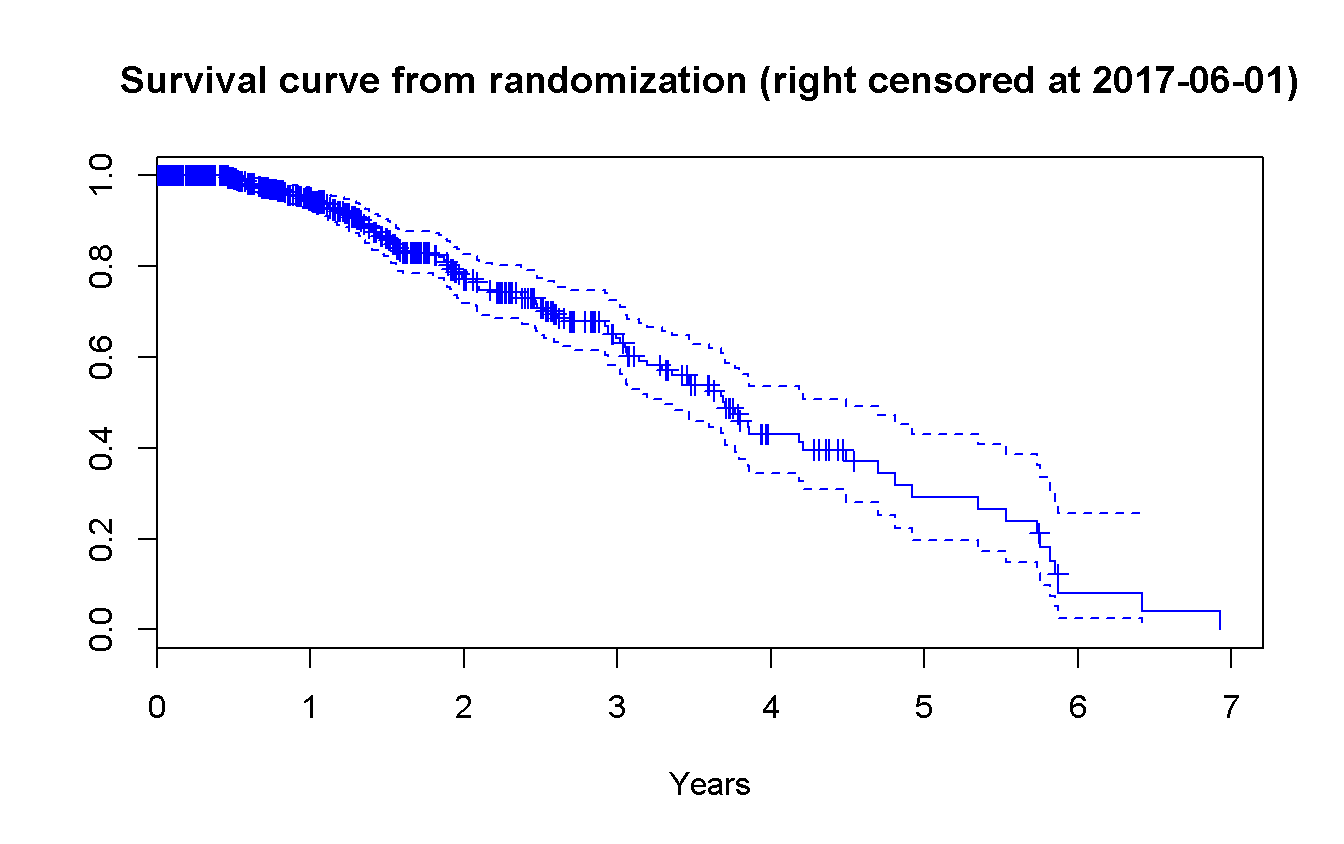
\includegraphics{SuDACDa-notes_files/figure-latex/ex_surv_curves-1.pdf}

\chapter*{Software}\label{software}
\addcontentsline{toc}{chapter}{Software}

\section{Packages}\label{packages}

All the exercise are solved using R (ver. 3.4.2) has been used provided
with packages: \texttt{survival} (\citet{R-survival}) for the survival
data analyses (reference package), \texttt{survminer}
(\citet{R-survminer}) for advance survival plot using \texttt{ggplot2}
(\citet{R-ggplot2}) package, \texttt{rms} (\citet{R-rms}) for additional
features on regression modeling strategies (survival ones included).

With regards to the data management, the collection of package
\texttt{tidyverse} (\citet{R-tidyverse}) is loaded, which includes:
\texttt{dplyr} (\citet{R-dplyr}) for data manipulation, \texttt{purrr}
(\citet{R-purrr}) for functional programming, \texttt{readr} (R-readr)
for data import, \texttt{tidyr} (R-tidyr) for funtions to tidy the data,
\texttt{tibble} (R-tibble) to take advantage of the \emph{tible} data
frame class and \texttt{ggplot2} as a interface for the Gramar of
Grahics.

The present book was written in RMarkdown (R-rmarkdown), compiled using
\texttt{knitr} (\citet{R-knitr}) and rendered as an HTML book by
\texttt{bookdown} (\citet{R-bookdown}).

\section{System Information}\label{system-information}

All the code is compiled on a system with the following overall
characteristics and loaded packages.

\begin{Shaded}
\begin{Highlighting}[]
\NormalTok{devtools::}\KeywordTok{session_info}\NormalTok{()}
\end{Highlighting}
\end{Shaded}

\begin{verbatim}
##  setting  value                       
##  version  R version 3.4.2 (2017-09-28)
##  system   x86_64, mingw32             
##  ui       RTerm                       
##  language (EN)                        
##  collate  English_United States.1252  
##  tz       Europe/Berlin               
##  date     2017-10-03                  
## 
##  package      * version date       source        
##  acepack        1.4.1   2016-10-29 CRAN (R 3.4.1)
##  assertthat     0.2.0   2017-04-11 CRAN (R 3.4.1)
##  backports      1.1.0   2017-05-22 CRAN (R 3.4.0)
##  base         * 3.4.2   2017-09-28 local         
##  base64enc      0.1-3   2015-07-28 CRAN (R 3.4.0)
##  bindr          0.1     2016-11-13 CRAN (R 3.4.1)
##  bindrcpp       0.2     2017-06-17 CRAN (R 3.4.1)
##  bookdown       0.5     2017-08-20 CRAN (R 3.4.1)
##  broom          0.4.2   2017-02-13 CRAN (R 3.4.0)
##  cellranger     1.1.0   2016-07-27 CRAN (R 3.4.1)
##  checkmate      1.8.3   2017-07-03 CRAN (R 3.4.1)
##  cluster        2.0.6   2017-03-16 CRAN (R 3.4.1)
##  cmprsk         2.2-7   2014-06-17 CRAN (R 3.4.1)
##  codetools      0.2-15  2016-10-05 CRAN (R 3.4.0)
##  colorspace     1.3-2   2016-12-14 CRAN (R 3.4.1)
##  compiler       3.4.2   2017-09-28 local         
##  data.table     1.10.4  2017-02-01 CRAN (R 3.4.0)
##  datasets     * 3.4.2   2017-09-28 local         
##  devtools       1.13.3  2017-08-02 CRAN (R 3.4.1)
##  digest         0.6.12  2017-01-27 CRAN (R 3.4.1)
##  dplyr        * 0.7.3   2017-09-09 CRAN (R 3.4.1)
##  evaluate       0.10.1  2017-06-24 CRAN (R 3.4.1)
##  forcats        0.2.0   2017-01-23 CRAN (R 3.4.1)
##  foreign        0.8-69  2017-06-21 CRAN (R 3.4.0)
##  Formula      * 1.2-2   2017-07-10 CRAN (R 3.4.1)
##  ggplot2      * 2.2.1   2016-12-30 CRAN (R 3.4.1)
##  ggpubr       * 0.1.5   2017-08-22 CRAN (R 3.4.1)
##  glue           1.1.1   2017-06-21 CRAN (R 3.4.1)
##  graphics     * 3.4.2   2017-09-28 local         
##  grDevices    * 3.4.2   2017-09-28 local         
##  grid           3.4.2   2017-09-28 local         
##  gridExtra      2.3     2017-09-09 CRAN (R 3.4.1)
##  gtable         0.2.0   2016-02-26 CRAN (R 3.4.1)
##  haven          1.1.0   2017-07-09 CRAN (R 3.4.1)
##  Hmisc        * 4.0-3   2017-05-02 CRAN (R 3.4.1)
##  hms            0.3     2016-11-22 CRAN (R 3.4.1)
##  htmlTable      1.9     2017-01-26 CRAN (R 3.4.1)
##  htmltools      0.3.6   2017-04-28 CRAN (R 3.4.1)
##  htmlwidgets    0.9     2017-07-10 CRAN (R 3.4.1)
##  httr           1.3.1   2017-08-20 CRAN (R 3.4.1)
##  jsonlite       1.5     2017-06-01 CRAN (R 3.4.1)
##  km.ci          0.5-2   2009-08-30 CRAN (R 3.4.1)
##  KMsurv         0.1-5   2012-12-03 CRAN (R 3.4.0)
##  knitr          1.17    2017-08-10 CRAN (R 3.4.1)
##  labeling       0.3     2014-08-23 CRAN (R 3.4.0)
##  lattice      * 0.20-35 2017-03-25 CRAN (R 3.4.1)
##  latticeExtra   0.6-28  2016-02-09 CRAN (R 3.4.1)
##  lazyeval       0.2.0   2016-06-12 CRAN (R 3.4.1)
##  lubridate      1.6.0   2016-09-13 CRAN (R 3.4.1)
##  magrittr     * 1.5     2014-11-22 CRAN (R 3.4.1)
##  MASS           7.3-47  2017-04-21 CRAN (R 3.4.1)
##  Matrix         1.2-11  2017-08-16 CRAN (R 3.4.1)
##  MatrixModels   0.4-1   2015-08-22 CRAN (R 3.4.1)
##  memoise        1.1.0   2017-04-21 CRAN (R 3.4.1)
##  methods      * 3.4.2   2017-09-28 local         
##  mnormt         1.5-5   2016-10-15 CRAN (R 3.4.0)
##  modelr         0.1.1   2017-07-24 CRAN (R 3.4.1)
##  multcomp       1.4-7   2017-09-07 CRAN (R 3.4.1)
##  munsell        0.4.3   2016-02-13 CRAN (R 3.4.1)
##  mvtnorm        1.0-6   2017-03-02 CRAN (R 3.4.0)
##  nlme           3.1-131 2017-02-06 CRAN (R 3.4.1)
##  nnet           7.3-12  2016-02-02 CRAN (R 3.4.1)
##  parallel       3.4.2   2017-09-28 local         
##  pkgconfig      2.0.1   2017-03-21 CRAN (R 3.4.1)
##  plyr           1.8.4   2016-06-08 CRAN (R 3.4.1)
##  polspline      1.1.12  2015-07-14 CRAN (R 3.4.0)
##  psych          1.7.8   2017-09-09 CRAN (R 3.4.1)
##  purrr        * 0.2.3   2017-08-02 CRAN (R 3.4.1)
##  quantreg       5.33    2017-04-18 CRAN (R 3.4.1)
##  R6             2.2.2   2017-06-17 CRAN (R 3.4.1)
##  RColorBrewer   1.1-2   2014-12-07 CRAN (R 3.4.0)
##  Rcpp           0.12.12 2017-07-15 CRAN (R 3.4.1)
##  readr        * 1.1.1   2017-05-16 CRAN (R 3.4.1)
##  readxl         1.0.0   2017-04-18 CRAN (R 3.4.1)
##  reshape2       1.4.2   2016-10-22 CRAN (R 3.4.1)
##  rlang          0.1.2   2017-08-09 CRAN (R 3.4.1)
##  rmarkdown      1.6     2017-06-15 CRAN (R 3.4.1)
##  rms          * 5.1-1   2017-05-03 CRAN (R 3.4.1)
##  rpart          4.1-11  2017-04-21 CRAN (R 3.4.1)
##  rprojroot      1.2     2017-01-16 CRAN (R 3.4.1)
##  rstudioapi     0.7     2017-09-07 CRAN (R 3.4.1)
##  rvest          0.3.2   2016-06-17 CRAN (R 3.4.1)
##  sandwich       2.4-0   2017-07-26 CRAN (R 3.4.1)
##  scales         0.5.0   2017-08-24 CRAN (R 3.4.1)
##  SparseM      * 1.77    2017-04-23 CRAN (R 3.4.0)
##  splines        3.4.2   2017-09-28 local         
##  stats        * 3.4.2   2017-09-28 local         
##  stringi        1.1.5   2017-04-07 CRAN (R 3.4.0)
##  stringr        1.2.0   2017-02-18 CRAN (R 3.4.1)
##  survival     * 2.41-3  2017-04-04 CRAN (R 3.4.1)
##  survminer    * 0.4.0   2017-06-07 CRAN (R 3.4.1)
##  survMisc       0.5.4   2016-11-23 CRAN (R 3.4.1)
##  TH.data        1.0-8   2017-01-23 CRAN (R 3.4.1)
##  tibble       * 1.3.4   2017-08-22 CRAN (R 3.4.1)
##  tidyr        * 0.7.1   2017-09-01 CRAN (R 3.4.1)
##  tidyverse    * 1.1.1   2017-01-27 CRAN (R 3.4.1)
##  tools          3.4.2   2017-09-28 local         
##  utils        * 3.4.2   2017-09-28 local         
##  withr          2.0.0   2017-07-28 CRAN (R 3.4.1)
##  xml2           1.1.1   2017-01-24 CRAN (R 3.4.1)
##  xtable         1.8-2   2016-02-05 CRAN (R 3.4.1)
##  yaml           2.1.14  2016-11-12 CRAN (R 3.4.1)
##  zoo            1.8-0   2017-04-12 CRAN (R 3.4.1)
\end{verbatim}

\bibliography{packages,book}


\end{document}
